\chapter{Modelling yeast biosynthesis strategies under constraints}
\label{ch:model}

To better understand the mechanistic basis of the YMC, I sought to build a model of how the cyclic sequence of cellular events responds to extracellular nutrient conditions.
However, it is challenging to develop a fine-grained model for the aspects of the YMC,
especially if the detailed molecular mechanisms are unclear.
Further complicating the development of a fine-grained model is the fact that the main read-outs from single-cell studies --- NAD(P)H and flavin autofluorescence --- are aggregate signals from several biochemical phenomena.

Thus, it is more feasible to construct coarse-grained models to answer biological questions about the YMC\@.
One such question is whether a finite proteome is responsible for the sequence of events in the yeast metabolic cycle, especially considering the high energetic and resource requirements of protein synthesis \parencite{oneillEukaryoticCellBiology2020,zylstraMetabolicDynamicsCell2022}.

Here, I use a genome-scale metabolic model and flux balance analysis (FBA) to address whether cellular events in the metabolic cycle reflect a strategy in resource allocation that optimises growth.

\pagebreak

Specifically, I aim to evaluate these hypotheses:
\begin{enumerate}
  \item A finite proteome pool gives rise to sequential scheduling of the synthesis of biomass components during growth: lipids, carbohydrates, amino acids, and nucleic acids.
        In other words, as an adaption, the cell synthesises biomass components in sequence rather than in parallel.
        This would explain the timing of biosynthetic events in the phases of the yeast metabolic cycle.
  \item This resource allocation strategy remains advantageous in many nutrient conditions and deletion strains,
        which would explain the robustness of the yeast metabolic cycle.
  \item Synthesis of biomass components in parallel, as opposed to in sequence, may be advantageous if the processes of synthesising each biomass component share similar enzyme levels across biomass components.
\end{enumerate}

\section{Introduction to flux balance analysis}
\label{sec:model-fba}

Metabolic network reconstructions are mathematical representations of a set of metabolic pathways in a living organism.
Usually, each metabolite is represented as a node, and metabolites are connected to each other through reactions that are represented as links \parencite{palssonSystemsBiologyConstraintbased2015}.
This information can be represented in a two-dimensional stoichiometric matrix, in which the rows of the matrix represent the metabolites, the columns represent the reactions, and the values of each element in the matrix show the stoichiometry of the reactions in the system.

For example, if reaction $R_{1}$ is defined by:

\begin{equation}
  \ce{1 M1 + 2 M2 -> 3 M3}
  \label{eq:model-example-chemical-reaction}
\end{equation}

the elements in the stoichiometric matrix that correspond to the metabolite-reaction combinations $(M_{1}, R_{1})$, $(M_{2}, R_{1})$, and $(M_{3}, R_{1})$ are -1, -2, and 3, respectively.

A genome-scale metabolic model is, in simple terms, a metabolic network reconstruction that aims to cover every biochemical reaction in a living system that is catalysed by a gene-encoded enzyme.
In most of the reactions represented in a metabolic network reconstruction, one or more chemical species react to create a different set of chemical species as products.
However, reactions in a metabolic network reconstruction may include processes that are not chemical reactions.
Such processes may include exchange of nutrients, as well as a reaction that models biomass formation.

Flux balance analysis (FBA) is a mathematical method that finds the steady-state flux of reactions through a metabolic network that is best for a given condition \parencite{orthWhatFluxBalance2010}.
These metabolic fluxes represent rates of chemical reactions.
At its core, FBA is a method of solving the linear programming problem of finding the flux values that optimise the output value of an objective function, subject to biological constraints.

Mathematically, the linear programming problem of FBA can be expressed as:

\begin{equation}
  \max \mathbf{c}^{\intercal} \mathbf{v}
  \label{eq:model-fba-objective}
\end{equation}

subject to

\begin{equation}
  \begin{gathered}
    \mathbf{S} \mathbf{v} = \mathbf{0}\\
    v_{i,\mathrm{min}} \leq v_{i} \leq v_{i,\mathrm{max}}
  \end{gathered}
  \label{eq:model-fba-constraints}
\end{equation}

where $\mathbf{c}$ is a vector of weights such that $\mathbf{c}^{\intercal} \mathbf{v}$ defines the objective function, $\mathbf{S}$ is the stoichiometric matrix, and $\mathbf{v}$ is the vector of fluxes. The expression $v_{i,\mathrm{min}}$ represents the lower bound and $v_{i,\mathrm{max}}$ represents the upper bound for each flux $v_{i}$ in $\mathbf{v}$.

The objective function is given as the task of maximising a mathematical expression that is based on a subset of fluxes (Eq.\ \ref{eq:model-fba-objective}).
Most commonly, the objective function is maximising the flux of the biomass reaction, thus optimising the growth rate of the cell.
The constraints for FBA are, in the most basic case, imposed by two factors:
the stoichiometric matrix and reaction flux bounds (Eq.\ \ref{eq:model-fba-constraints}).
The stoichiometric matrix balances reaction inputs and outputs, while flux bounds impose upper and lower limits on the fluxes of each reaction.
These constraints restrict the solution space for the FBA problem.

FBA thus offers a computationally inexpensive way to simulate metabolism in a living system, as opposed to solving a large set of differential equations that describe the kinetics of biochemical reactions.
Such differential equations can be difficult to construct and parametrise.

\section{Modelling temporal scheduling of biosynthesis}
\label{sec:model-temporal}

Previous studies have attempted to use FBA to model how each phase of the YMC has different metabolic requirements.
\textcite{takhaveevTemporalSegregationBiosynthetic2023} showed that in different stages of the cell division cycle, the cell synthesises different components of its biomass at different levels.
In the study, they blocked synthesis of each class of macromolecule and recorded the changes in single-cell NAD(P)H cycles, representing the YMC, to quantify the level of each class of macromolecule that the cell synthesises at each time point within a cell division cycle.
Then, they used these activities as coefficients for a modified thermodynamic-stoichiometric metabolic model at each time point and used FBA to deduce biomass production rates.
% Does not suggest that synthesis of each class of macromolecule excludes all others (which makes sense).
% Rather, this study confirms that timescale of observed synthesis events matches simulations.
% Do I even cite this?  It's so bad.
Additionally, \textcite{cesurGenomeWideAnalysisYeast} constructed a different FBA model for each YMC phase based on transcriptomic and epigenetic data.
They did so using the GIMME algorithm \parencite{beckerContextSpecificMetabolicNetworks2008}, which excludes reactions that correspond to genes that are not expressed at certain time points.
Both studies model the metabolic state of the cell at each phase of the YMC, rather than predicting the time the cell takes to replicate or to synthesise biomass components.

An attempt in extending FBA to solve a time-dependent resource allocation problem was \textcite{reimersCellularTradeoffsOptimal2017}.
This study extended a genome-scale model of the cyanobacterium \textit{Synechococcus elongatus} PCC7942 to find the temporal order of intracellular synthesis reactions which optimises the growth rate of the cell, under resource constraints.
However, extending the ideas in \textcite{reimersCellularTradeoffsOptimal2017} to the study of the YMC is hampered by the lack of an explicit mechanistic model of the YMC, owing to the unknowns of the biochemical mechanisms of the YMC\@.
Instead, any FBA model based on the metabolic model must include a phenomenological description of a metabolic cycle, which would be equivalent to including an external oscillator as implemented by \textcite{reimersCellularTradeoffsOptimal2017} as a light-dark cycle.

Traditional genome-scale models assume that the uptake rate of carbon source limits production.
However, levels of each enzyme also restrict reaction fluxes, leading to the development of enzyme-constrained models.
An enzyme-constrained model fits the assumption that there is a fixed number of amino acids the cell has to distribute \parencite{weisseMechanisticLinksCellular2015}.
Models like \textcite{sanchezImprovingPhenotypePredictions2017} and \textcite{elsemmanWholecellModelingYeast2022} constrain the total sum of fluxes based on a defined total amount of enzyme.
\textcite{elsemmanWholecellModelingYeast2022} additionally imposed a ribosome capacity constraint and compartment constraints.

In this chapter, I used an enzyme-constrained genome-scale model of \textit{Saccharomyces cerevisiae} and performed FBA to simulate two strategies of scheduling of the synthesis of biomass components: in sequence and in parallel.
To simulate the cell prioritising the synthesis of each biomass component in sequence, I ablated metabolites from the biomass reaction so that one biomass component remained, then optimised the model.
To assess the advantage of sequential synthesis over parallel synthesis, I estimated the synthesis time for each biomass component based on ablation, then compared these times predicted by the unmodified model.
To show that sequential synthesis is an adaptation for a finite proteome pool, I varied the size of the enzyme-available proteome pool to observe its effect on the cell's preferred scheduling strategy.
Finally, to show how nutrient conditions affect the cell's scheduling strategy, I modelled changes in carbon and nitrogen source concentrations, then observed how the changes affect allocation of the proteome to metabolic enzymes.


\section{The Yeast8 and ecYeast8 models and their formalisms}
\label{sec:model-yeast8}

To impose proteome constraints, I used the enzyme-constrained Yeast8 (ecYeast8) model \parencite{luConsensusCerevisiaeMetabolic2019} and performed FBA\@.
I used this model because it is recent, offers a good coverage of reactions, and is continuously updated in a well-characterised and well-documented software repository.
Here, I used the model ec\-Yeast\-8.6.0, the latest version for which both original and enzyme-constrained variants are available.
ecYeast8 uses the GECKO formalism \parencite{sanchezImprovingPhenotypePredictions2017} --- specifically, GECKO 2 \parencite{domenzainReconstructionCatalogueGenomescale2022}, the latest published version.
GECKO applies an enzyme constraint by modifying the stoichiometric matrix of a genome-scale metabolic model.
In addition, the model has `pseudometabolites' defined by reactions that group specific chemical species in general classes.
These formalisms allow studying each class of biomass component (e.g.\ lipid, protein, carbohydrate) individually (Methods Section~\ref{subsec:methods-fba-ecYeast8}).


\subsection{GECKO}
\label{subsec:model-yeast8-gecko}

In a conventional genome-scale model, metabolic fluxes through reactions are constrained by lower and upper bounds.
This constraint narrows the solution space when the objective function is optimised.
GECKO imposes an additional constraint on the metabolic fluxes based on the concentration of the enzyme that catalyses the reaction (Fig.\ \ref{fig:model-gecko}).

\begin{figure}[hb!]
  \centering
  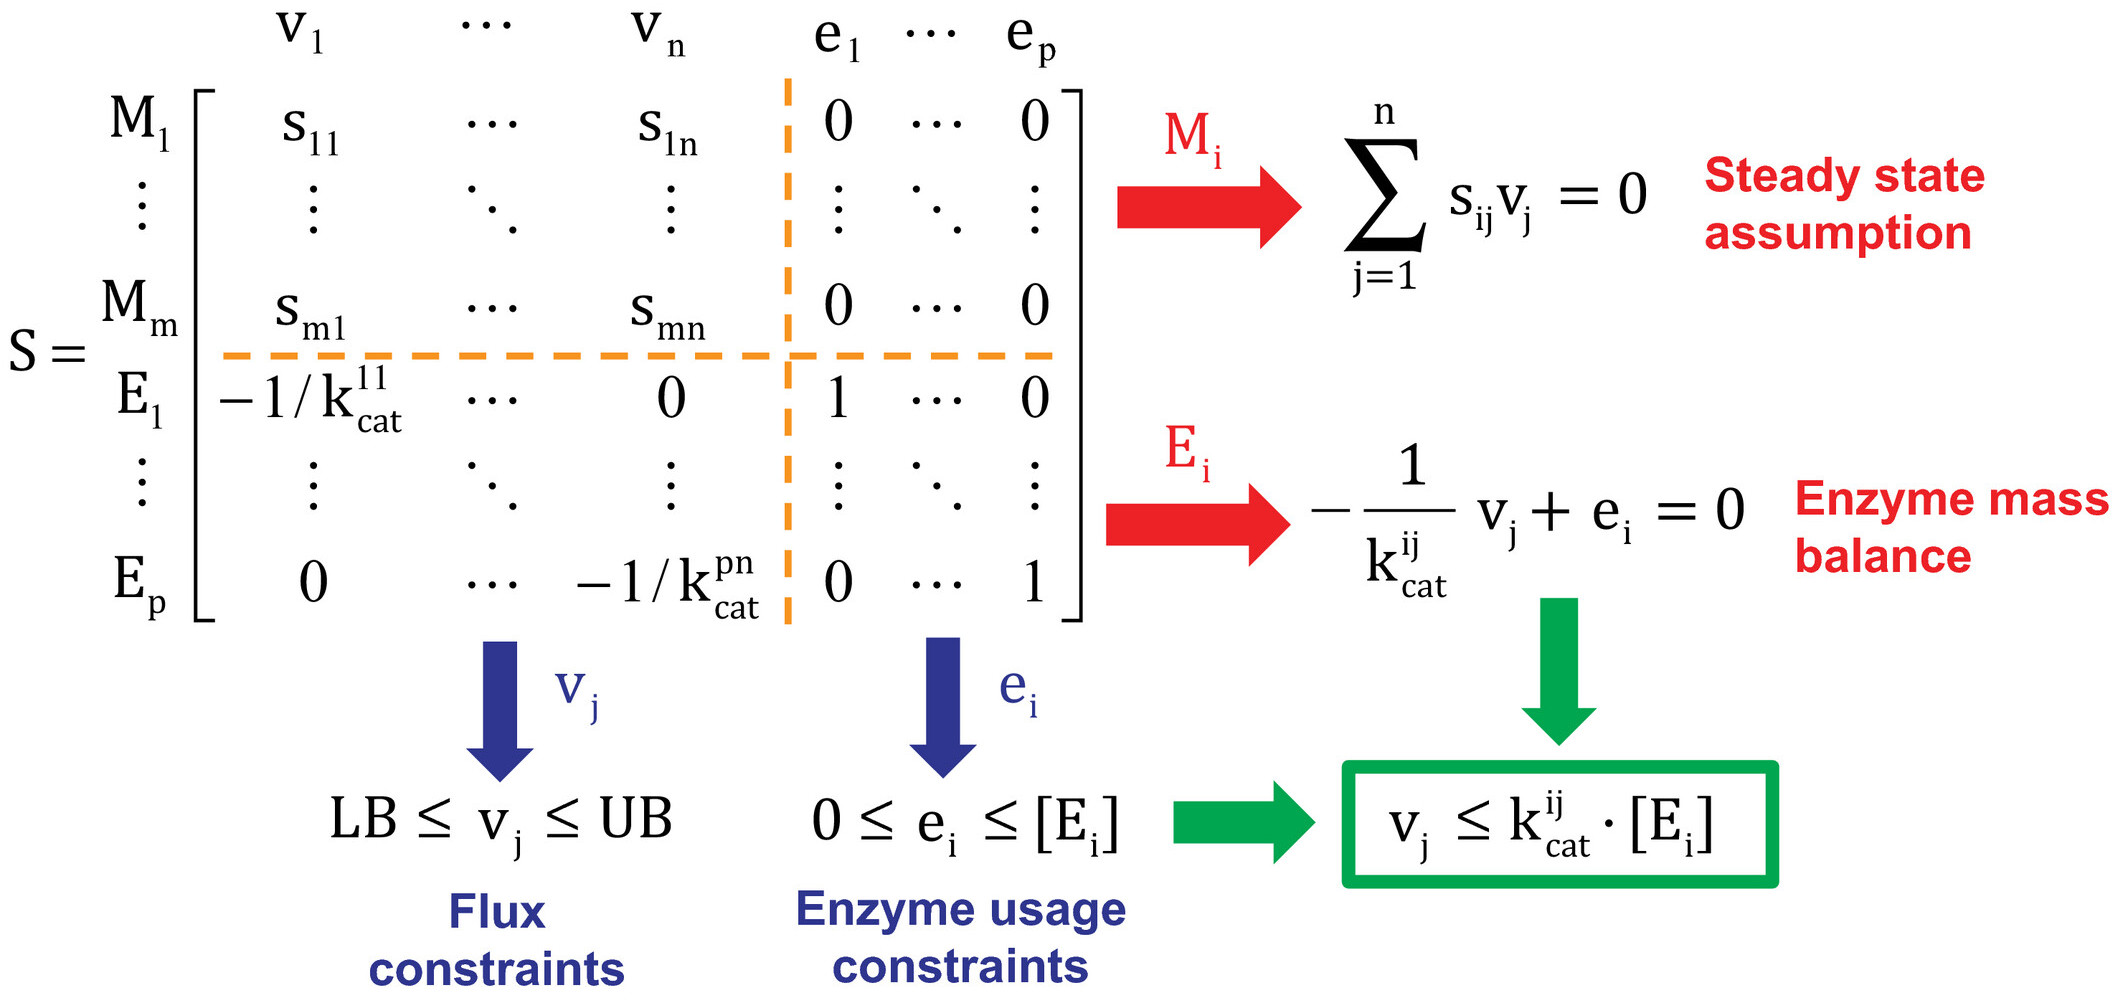
\includegraphics[width=0.9\linewidth]{sanchezImprovingPhenotypePredictions2017_1b_adapted}
  \caption[
    Modifications to the stoichiometric matrix of a genome-scale model that GECKO imposes
  ]{
    Modifications to the stoichiometric matrix of a genome-scale model that GECKO imposes.
    The original stoichiometric matrix $\mathbf{S}$ includes metabolites $M_{1} \ldots M_{m}$ and reactions $v_{1} \ldots v_{n}$.
    GECKO extends this matrix to include enzymes $E_{1} \ldots E_{p}$ and enzyme usage reactions $e_{1} \ldots e_{p}$.
    The new stoichiometric matrix can be seen as four submatrices concatenated together: the upper left submatrix is the original $\mathbf{S}$, the upper right submatrix is $\mathbf{0}$, the lower left submatrix encodes kinetic information, and the lower right submatrix is $\mathbf{I}$.
    Figure adapted from~\textcite{sanchezImprovingPhenotypePredictions2017}.
  }
  \label{fig:model-gecko}
\end{figure}

GECKO modifies the linear programming of FBA as defined by Eq.\ \ref{eq:model-fba-objective} and~\ref{eq:model-fba-constraints} so that enzymes are expressed as metabolites that take part in reactions.
This can be expressed as:

\begin{equation}
  \max \mathbf{c}^{\intercal} \mathbf{v}
  \label{eq:model-gecko-fba-objective}
\end{equation}

subject to

\begin{equation}
  \begin{gathered}
    \mathbf{S} \mathbf{v} = \mathbf{0}\\
    v_{j,\mathrm{min}} \leq v_{j} \leq v_{j,\mathrm{max}}\\
    v_{j} \leq k_{\mathrm{cat}}^{ij} \cdot [E_{i}]
  \end{gathered}
  \label{eq:model-gecko-fba-constraints}
\end{equation}

where $v_{j}$ is the flux of each reaction $R_{j}$ catalysed by enzyme $E_{i}$, $k_{\mathrm{cat}}^{ij}$ is the catalytic constant of the enzyme $E_{i}$ for reaction $R_{j}$, and $[E_{i}]$ represents the concentration of the enzyme $E_{i}$.
These constraints ensure that each $v_{j}$ does not exceed the $v_{\mathrm{max}}$ of $E_{i}$.
Each enzyme $E_{i}$ may catalyse one or more reactions $R_{j}$.
Appendices~\ref{append:model-gecko}--\ref{append:model-gecko-nonsimple} illustrate these modifications by considering how they modify chemical reactions in the model.

% The constraints in Eq.\ \ref{eq:model-gecko-fba-constraints} is imposed by extending the stoichiometric matrix $\mathbf{S}$ and flux vector $\mathbf{v}$.
% Specifically, $\mathbf{S}$ has additional rows to represent new metabolites that represent each enzyme $E_{i}$.
% The matrix $\mathbf{S}$ also has additional columns for new reactions $ER_{i}$ that model enzyme usage and for a new reaction $ER_{\mathrm{pool}}$ that models a limited proteome pool.
% Kinetic information in the form of $k_{\mathrm{cat}}^{ij}$ values are included as elements in the extended stoichiometric matrix.
% Finally, $\mathbf{v}$ has additional elements that correspond to the additional columns of $\mathbf{S}$.

% The constraint $v_{j} \leq k_{\mathrm{cat}}^{ij} \cdot [E_{i}]$ from Eq.\ \ref{eq:model-gecko-fba-constraints} can be expressed as:

% \begin{equation}
%   \begin{gathered}
%     -\frac{1}{k_{\mathrm{cat}}^{ij}}v_{j} + e_{i} = 0\\
%     0 \leq e_{i} \leq [E_{i}]
%   \end{gathered}
%   \label{eq:model-gecko-fba-constraints-extended}
% \end{equation}

% where $e_{i}$ represents the flux of an enzyme usage reaction $ER_{i}$ associated with $E_{i}$.


\section{Ablating pseudometabolites from the biomass reaction}
\label{sec:model-yeast8-pseudometabolites}

\subsection{Definition of ablation}
\label{sec:model-yeast8-pseudometabolites-def}

To simulate producing each class of biomass component in turn,
I took advantage of pseudometabolites in ecYeast8 to remove them in turn from the biomass reaction ---
in other words, ablating pseudometabolites from the biomass reaction.
%Specifically, I exclude each pseudometabolite from the biomass reaction, in turn, and optimise the model.

Consider the objective function, the biomass reaction:

\texttt{
  47.5883 atp\_c + 47.5883 h2o\_c + lipid\_c + protein\_c + carbohydrate\_c\\
  + dna\_c + rna\_c + cofactor + ion \\
  --> 47.5883 adp\_c + biomass\_c + 47.5883 h\_c + 47.5883 pi\_c
}

There are seven pseudometabolites: lipid, protein, carbohydrate, DNA, RNA, cofactor, and ion.

To simulate the cell prioritising biosynthesis of lipids, I set the stoichiometric coefficients of all pseudometabolites except for lipids to zero in the above equation, giving:

\texttt{
  47.5883 atp\_c + 47.5883 h2o\_c + lipid\_c \\
  --> 47.5883 adp\_c + biomass\_c + 47.5883 h\_c + 47.5883 pi\_c
}

Using this modified reaction as the objective function, the model was optimised using FBA, and
this process was repeated for the other pseudometabolites, resulting in different growth rates for each round of ablation (Fig.\ \ref{fig:model-ablate-fluxes}).

\begin{figure}[hb!]
  \centering
  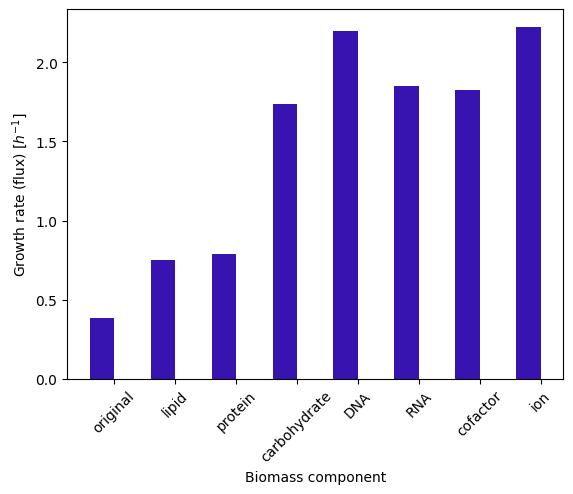
\includegraphics[width=.6\linewidth]{ablation_example_fluxes.png}
  \caption[
    Growth rates from the original model and from the ablated versions of the model
  ]{
    %Growth rates from the original model ($\gro$; leftmost bar) and from the ablated versions of the model ($\griabl$, where $i$ represents each biomass components among lipids, proteins, carbohydrates, DNA, RNA, cofactors, and ions; other bars)
    Growth rates from the original model (leftmost bar) and from the ablated versions of the model (other bars)
  }
  \label{fig:model-ablate-fluxes}
\end{figure}


\subsection{Effect of ablation on allocation of proteome to enzymes}
\label{sec:model-yeast8-pseudometabolites-allocation}

To assess whether ablation leads to metabolic changes that reflect cellular biochemistry, I quantified how proteome allocation to enzymes changes across rounds of ablation.
When the model prioritised a different biomass component in each round of ablation, the model partitioned the limited proteome available for enzyme production differently.
In other words, in each round of ablation, the vector of fluxes carried by each enzyme usage pseudoreaction (defined in Eq.\ \ref{eq:model-gecko-enzyme-usage}) was different from each other and from the non-ablated case, in which all biomass components were synthesised in parallel.

To quantify changes in proteome allocation across rounds of ablation, I computed the base-2 logarithm of fold changes of fluxes relative to the non-ablated, parallel case.
This computation is defined as:

\begin{equation}
  \log_{2}(\mathrm{FC}_{i,j}) = \log_{2}\left( \frac{e_{i,j}^{\prime}}{e_{i, \mathrm{par}}^{\prime}} \right)
  \label{eq:model-foldchange}
\end{equation}

where, to ensure that $\log_{2}(\mathrm{FC}_{i,j})$ can be defined for all $i$ and $j$,

\begin{equation}
  e^{\prime} =
  \begin{cases}
    \epsilon, & \text{if}\ |e|<\epsilon \\
    e, & \text{otherwise}
  \end{cases}
  \label{eq:model-epsilon-round}
\end{equation}

where $e^{\prime}$ is either $e_{i,j}^{\prime}$ or $e_{i, \mathrm{par}}^{\prime}$, $e$ is the corresponding $e_{i,j}$ or $e_{i, \mathrm{par}}$, and $\epsilon$ is the minimum flux of $\SI{1}{\molecule~\cell^{-1}} = \SI{1.11d-10}{\mmolgdw}$, computed assuming a cell dry weight of \SI{15}{\pico\gram} dry weight per cell \parencite{shermanGettingStartedYeast2002}.
Here, $e_{i, \mathrm{par}}$ represents the flux of an enzyme usage reaction associated with each enzyme $E_{i}$ in the model (defined in Eq.\ \ref{eq:model-gecko-enzyme-pool}) in the non-ablated, parallel case, and $e_{i,j}$ represents the flux of the enzyme usage reaction when biomass component $j$ is prioritised in a round of ablation.

% The value $\epsilon$ is defined as:

% \begin{equation}
%   \begin{aligned}
%     \epsilon &= \SI{1}{\molecule~\cell^{-1}~\hour^{-1}}\\
%              &= \frac{(\SI{1}{\molecule})}{(\SI{1}{\cell})(\SI{1}{\hour})} \cdot \frac{(\SI{1}{\cell})}{(\SI{15}{\pico\gram_{DW}})} \cdot \frac{(\SI{1}{\mol})}{(\SI{6.02214d23}{\molecule)}}\\
%              &= \SI{1.11d-13}{\mol~\gram_{DW}^{-1}~\hour^{-1}}\\
%              &= \SI{1.11d-10}{\mmolgdwh}\\
%   \end{aligned}
%   \label{eq:model-epsilon}
% \end{equation}

% assuming a reasonable minimum reaction flux of \SI{1}{\molecule~\cell^{-1}~\hour^{-1}} and a cell dry weight of \SI{15}{\pico\gram} dry weight per cell \parencite{shermanGettingStartedYeast2002}.

If $\log_{2}(\mathrm{FC}_{i,j}) > 0$, the cell allocates more of its proteome to produce enzyme $E_{i}$ when biomass component $j$ is prioritised; the reverse is true if $\log_{2}(\mathrm{FC}_{i,j}) < 0$.
In addition, if enzyme expression switches on ($e_{i, \mathrm{par}} = 0$), $\log_{2}(\mathrm{FC}_{i,j}) \ll 0$.
Conversely, if enzyme expression switches off ($e_{i, j} = 0$), $\log_{2}(\mathrm{FC}_{i,j}) \gg 0$.

% ON SECOND THOUGHT, THIS LOOKS LIKE UNNECESSARY DETAIL WHICH BELONGS IN THE METHODS/APPENDIX, AND POTENTIALLY CONFUSES PEOPLE.
% Subsystem information aids interpretation of the changes in proteome allocation across rounds of ablation.
% Here, I matched the flux carried by each enzyme usage pseudoreaction to the enzyme-catalysed reaction that the enzyme is associated with.
% If an enzyme usage pseudoreaction is associated with multiple enzyme-catalysed reactions, data entries were duplicated accordingly.
% Then, the subsystem associated with each enzyme-catalysed reaction was taken from the gene-protein map, and noted.

To show that the re-allocation of the proteome in each round of ablation reflects metabolic pathways that are relevant for prioritising the synthesis of the respective biomass component, Fig.\ \ref{fig:model-ablate-enz-use} categorises fold changes of enzyme-catalysed reactions by subsystem.

\begin{figure}
  \centering
  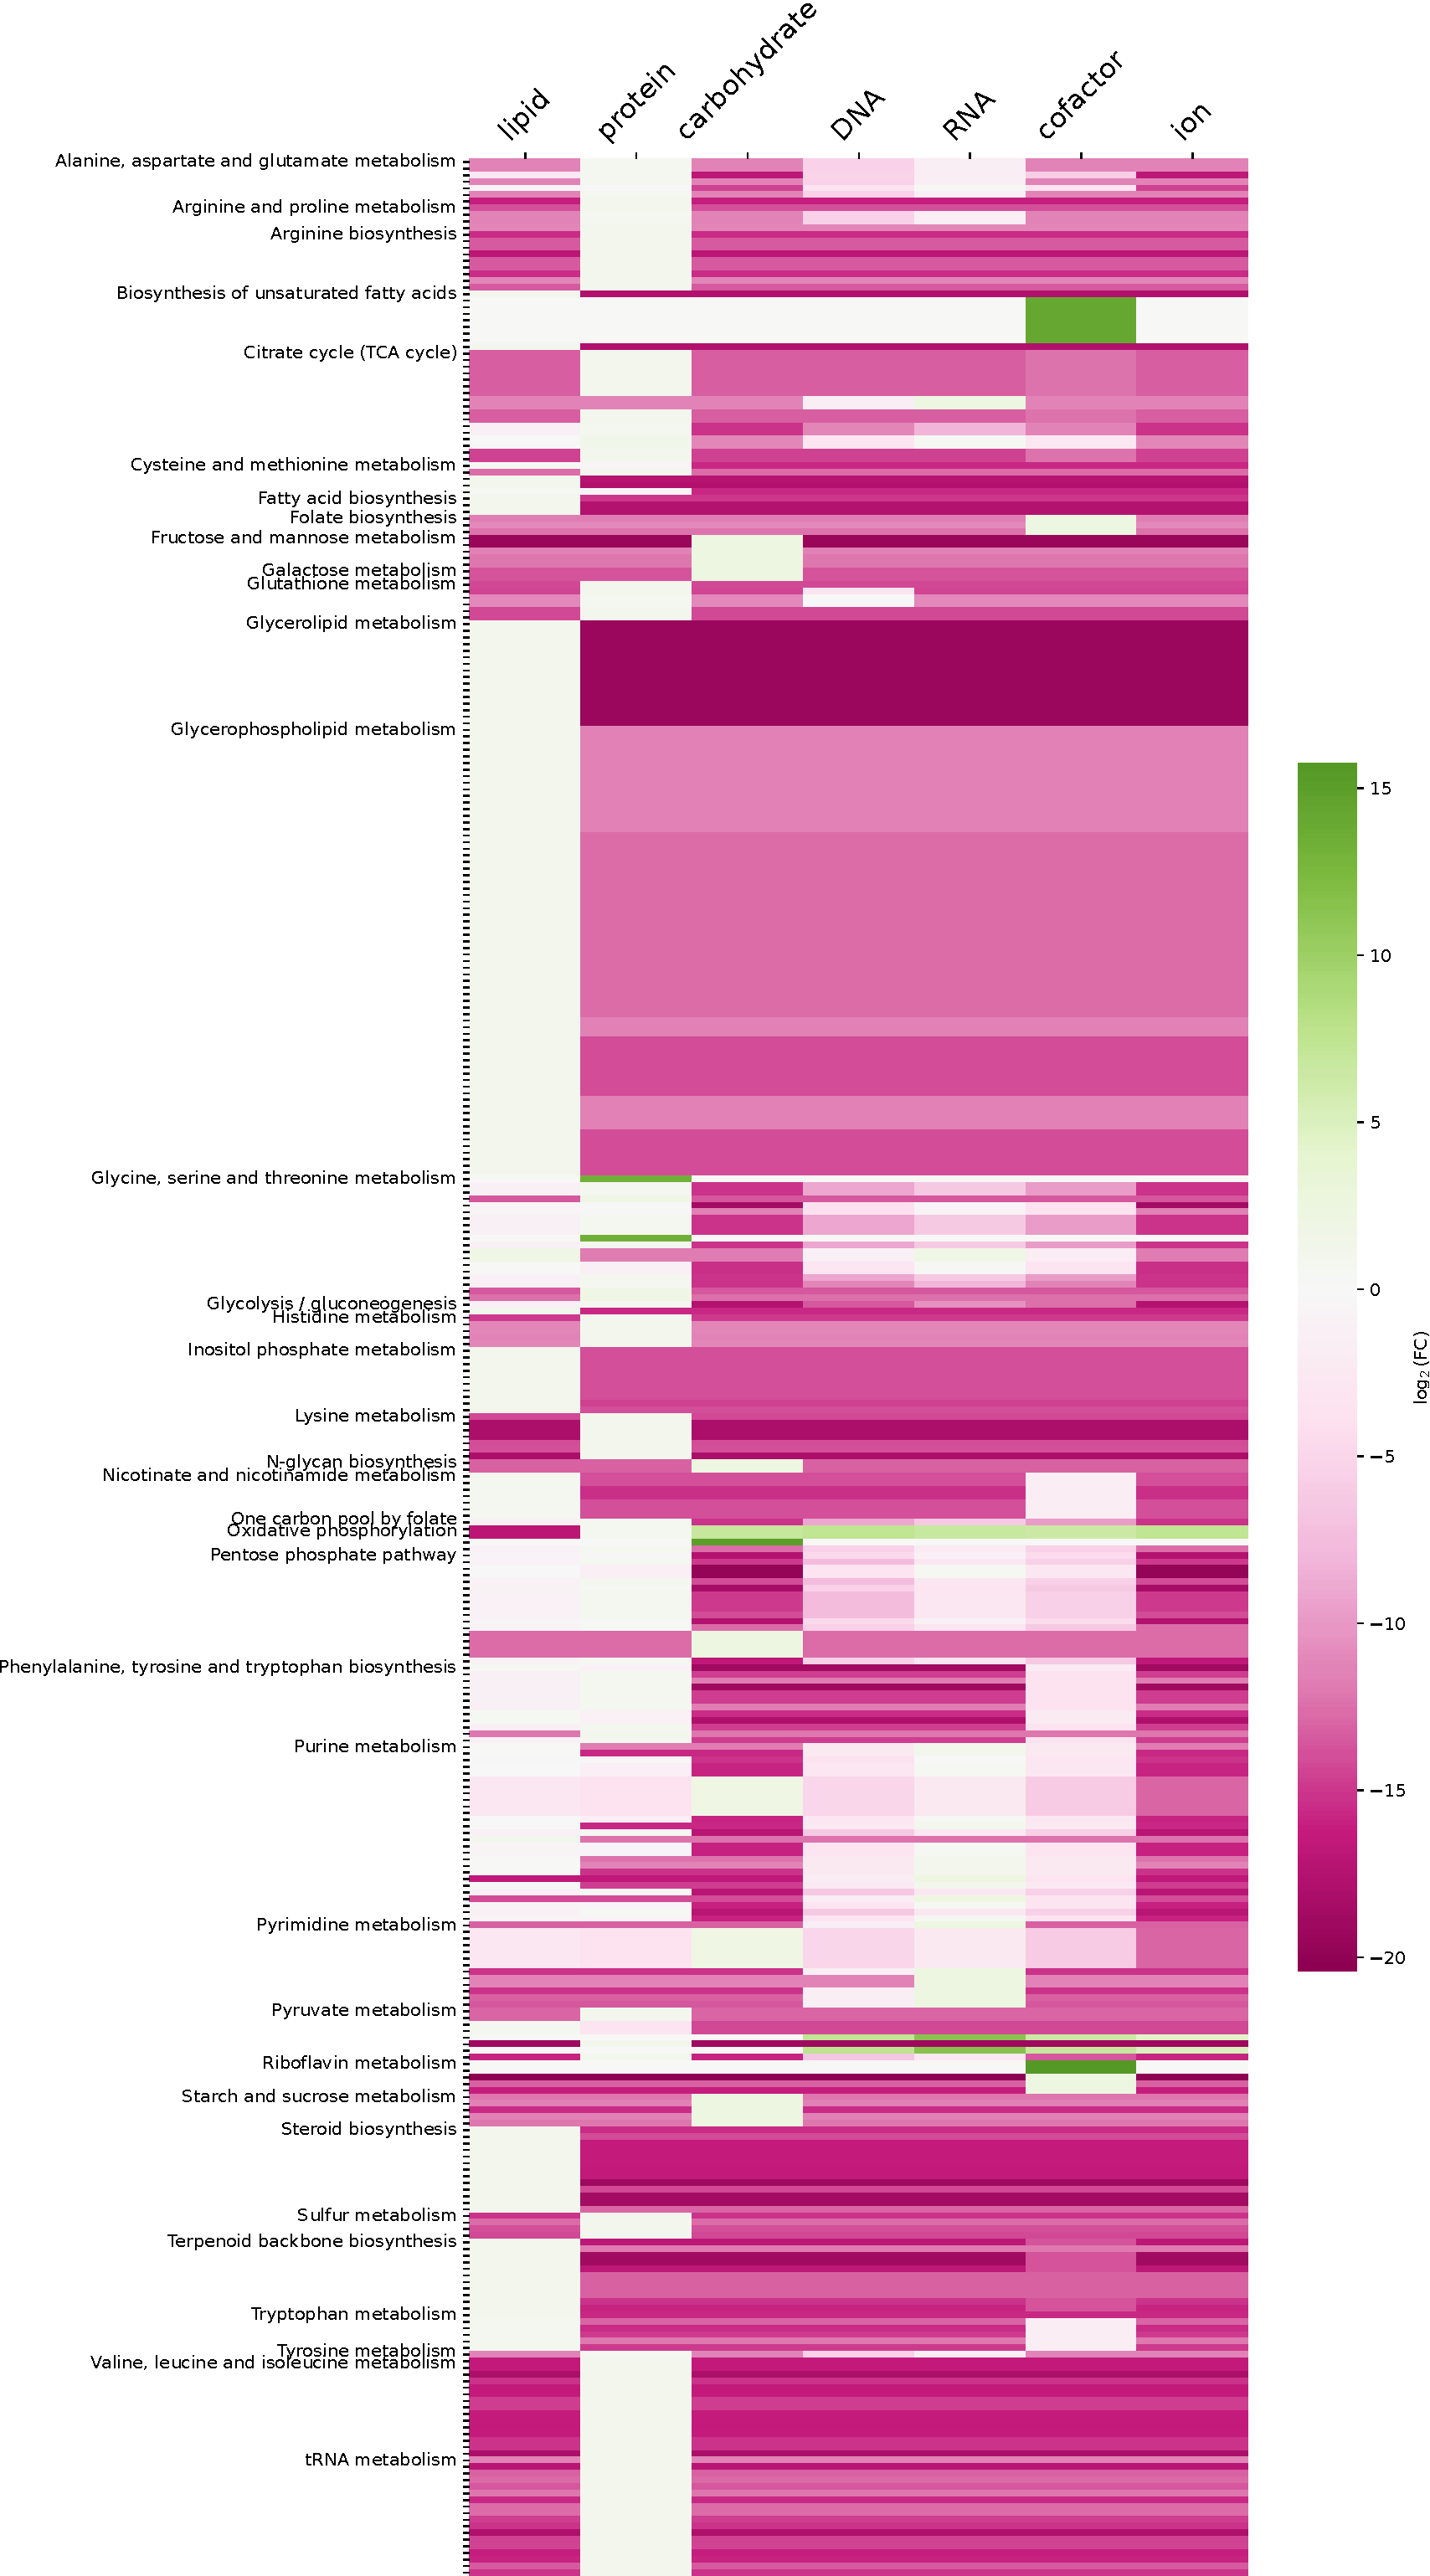
\includegraphics[width=.8\linewidth]{allocation_fc}
  \caption[
    $\log_{2}(\mathrm{FC})$ of enzyme usage reaction flux in rounds of ablation
  ]{
    $\log_{2}(\mathrm{FC})$ of enzyme usage reaction flux (Eq.\ \ref{eq:model-gecko-enzyme-usage}) in rounds of ablation, according to biomass component prioritised.
    %The cell changes how it allocates its proteome to enzymes when different components of its biomass are prioritised.
    Each column shows the component that remains in each round of pseudometabolite ablation (labels on top).
    Each row represents an enzyme, and rows are grouped by subsystem (labels on left).
    Colours represent $\log_{2}(\mathrm{FC})$ (defined in Eq.\ \ref{eq:model-foldchange}) showing how enzyme usage fluxes change in rounds of ablation: green shows an increase, while pink shows a decrease.
    Rows in which $|\log_{2}(\mathrm{FC})| < 11$ for all biomass components are not shown to restrict the number of reactions ($n = \num{3897}$) for visualisation.
  }
  \label{fig:model-ablate-enz-use}
\end{figure}

Specifically, the figure shows:
\begin{enumerate}
  \item When any biomass component was prioritised, the cell de-allocated its proteome to most of its enzymes, as $\log_{2}(\mathrm{FC}_{i,j}) < 0$ for most values of $i, j$.
        However, there were cases with strong increases in allocation ($\log_{2}(\mathrm{FC}_{i,j}) > 0$).
        For example, when cofactors were prioritised, there were strong increases in biosynthesis of unsaturated fatty acids and in riboflavin metabolism.
        Additionally, there were strong increases in oxidative phosphorylation when carbohydrate, DNA, RNA, cofactor, or ion was prioritised.
  \item When I modelled a cell that prioritises lipid biosynthesis, the model showed the least change relative to the parallel (non-ablated case), compared to other biomass components.
        The changes included increases of fluxes in the subsystems of fatty acid biosynthesis, glycerolipid metabolism, glycerophospholipid metabolism, inositol phosphate metabolism, steroid biosynthesis, and terpenoid backbone.
        Given that these subsystems are directly related to lipid metabolism, such changes were expected.
        In addition, during lipid biosynthesis, the model showed decreases of fluxes in oxidative phosphorylation, the TCA cycle, and in amino acid metabolism, with fluxes varying depending on the amino acid.
  \item When I modelled a cell that prioritises protein biosynthesis, the model showed small increases in fluxes associated with amino acid metabolism, tRNA metabolism, and oxidative phosphorylation.
        Such increases were expected as these led to production of substrates that are required for translation.
        Conversely, when other biomass components (carbohydrate, ion, DNA, RNA, and cofactor) were prioritised, there were decreases in fluxes in glycine, serine, and threonine metabolism.
  \item When I modelled a cell that prioritises carbohydrate biosynthesis, the model showed increases in fructose metabolism, mannose metabolism, N-glycan biosynthesis, and starch and sucrose metabolism.
        This was expected given that these reactions relate directly to pathways for synthesis of carbohydrates.
  \item When I modelled a cell that prioritises RNA biosynthesis, the model showed increases in the purine metabolism and pyrimidine metabolism subsystems, along with a mixed picture in the pentose phosphate pathway.
        The increases were expected given the presence of purines and pyrimidines in RNA and the role of the pentose phosphate pathway in generating the precursors for these compounds.
        However, these subsystems showed weak decreases in flux when DNA is prioritised, though the enzyme usage flux profile overall is similar to when RNA is prioritised.
\end{enumerate}

Because the changes of fluxes reflect cellular biochemistry, results thus validate ablation of biomass components as a method to simulate sequential synthesis of biomass components by the cell.


\section{Estimating timescale of biosynthesis}
\label{sec:model-timescale}

To evaluate whether sequential or parallel synthesis of biomass components offers a time advantage during cell growth, I estimated the timescale of biosynthesis for either resource allocation strategy (Fig.\ \ref{fig:model-ablate-times}).

\begin{figure}[htbp!]
  \centering
  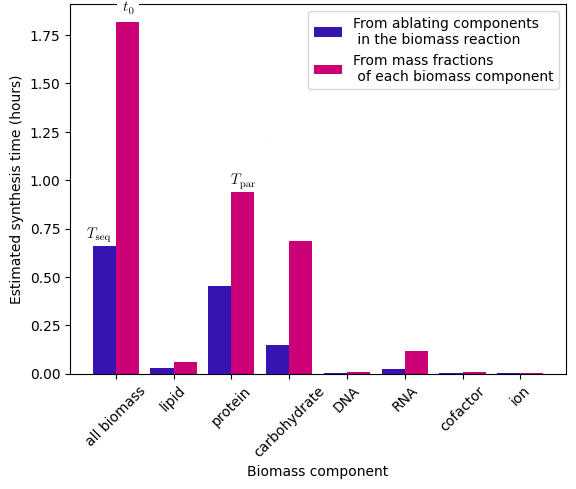
\includegraphics[width=.7\linewidth]{ablation_example_adapted.png}
  \caption[
    Estimated synthesis times of biomass components, from ablation and from scaling doubling time by mass fraction.
  ]{
    Estimated synthesis times of biomass components, from ablation (blue bars) and from scaling doubling time by mass fraction (red bars).
    Bars under `all biomass' indicate (blue) $\Tseq$ (defined in Eq.\ \ref{eq:model-a}) and (red) the doubling time $t_{0}$ (defined in Eq.\ \ref{eq:model-doubling-time}).
    Other bars indicate (blue) $\Tiabl$ (defined in Eq.\ \ref{eq:model-ablated-time}) and (red) $\Tiprop$ (defined in Eq.\ \ref{eq:model-proportional-time}); $\Tpar$ is the greatest $\Tiprop$.
  }
  \label{fig:model-ablate-times}
\end{figure}

Based on the objective function of the unmodified model, the doubling time was computed as follows:

\begin{equation}
  t_{0} = \frac{\ln 2}{\gro}
  \label{eq:model-doubling-time}
\end{equation}

where $t_{0}$ is the doubling time and $\gro$ is the growth rate, equivalent to the optimised flux of the biomass reaction.

Based on the growth rates computed in rounds of ablation (Fig.\ \ref{fig:model-ablate-fluxes}), the synthesis time of each biomass component was computed as follows:

\begin{equation}
  \Tiabl = f_{i} \cdot \frac{\ln 2}{\griabl}
  \label{eq:model-ablated-time}
\end{equation}

where
$i$ represents each of the biomass components (lipids, proteins, carbohydrates, DNA, RNA, cofactors, and ions),
$\Tiabl$ is the predicted time for synthesis of each biomass component,
$f_{i}$ is the mass fraction of each biomass component (Table~\ref{tab:model-biomfrac}), and
$\griabl$ is the optimal flux of the ablated biomass reaction.
In Eq.\ \ref{eq:model-ablated-time}, $f_{i}$ acts as a scaling factor so that the synthesis time of a biomass component is proportional to the proportion of the biomass component in dry cell mass.

For comparison, I computed estimates of the time for each biomass component, assuming that it is proportional to the mass fraction:

\begin{equation}
  \Tiprop = f_{i} \cdot t_{0}
  \label{eq:model-proportional-time}
\end{equation}

where $t_{0}$ is the doubling time found in Eq.\ \ref{eq:model-doubling-time}.

To determine whether sequential biosynthesis of biomass components or parallel biosynthesis of biomass components is advantageous, I defined a ratio $\ratioabl$ that represents the ratio between the total time predicted by ablation and the biomass component that is predicted to take the most time:

\begin{equation}
  \ratioabl = \frac{\Tseq}{\Tpar}
  \label{eq:model-ratio-simplified}
\end{equation}

where $\Tseq$ represents the predicted growth time assuming sequential biosynthesis and $\Tpar$ represents the limiting biomass synthesis time assuming parallel biosynthesis.

\pagebreak

The quantities $\Tseq$ and $\Tpar$ are defined:

\begin{equation}
  \Tseq = \sum_{i} \Tiabl %= \sum f_{i} \cdot \frac{\ln 2}{\griabl}
  \label{eq:model-a}
\end{equation}

% \begin{equation}
%   \begin{aligned}
%     \Tpar \coloneqq \argmax_{i} \Tiprop = \Tabl{protein} = \biomfrac{protein} \cdot \frac{\ln 2}{\gro},\\
%     \because \argmax_{i} f_{i} = \biomfrac{protein}
%   \end{aligned}
%   \label{eq:model-b}
% \end{equation}

\begin{equation}
  \Tpar = \argmax_{i} \Tiprop
  \label{eq:model-b}
\end{equation}

% I DON'T THINK THIS SENTENCE IS NEEDED IN LIGHT OF THE EXISTENCE OF THE THIRD LINE IN eq:model-ratio
%Because $\biomfrac{protein} = 0.525$ (Table~\ref{tab:model-biomfrac}), $\Tpar = \Tprop{protein}$.

Therefore,

\begin{equation}
  \begin{aligned}
    \ratioabl &= \frac{\Tseq}{\Tpar} \\
    & = \frac{\left( \sum_{i} \Tiabl \right)}{\left( \argmax_{i} \Tiprop \right)}\\
    & = \frac{\left(  \sum_{i} f_{i} \cdot \frac{\ln 2}{\griabl} \right)}{\left( \biomfrac{protein} \cdot \frac{\ln 2}{\gro} \right)}\\
    %& = \left( \sum_i \frac{f_i}{\griabl} \right) \cdot \frac{\gro}{\biomfrac{protein}} \\
    & = \left( \frac{\biomfrac{lipid}}{\grabl{lipid}} + \frac{\biomfrac{protein}}{\grabl{protein}} + \cdots + \frac{\biomfrac{ion}}{\grabl{ion}} \right) \cdot \frac{\gro}{\biomfrac{protein}}
    \end{aligned}
  \label{eq:model-ratio}
\end{equation}

The expression in Eq.\ \ref{eq:model-ratio} means that the definition of the $\ratioabl$ ratio does not reduce to a trivial expression and depends on the $\gro$ and the $\griabl$ values, which are independent of each other.
%This relationship between $\ratioabl$ and $\gro$ and $\griabl$ is explored in section~\ref{sec:model-pool}.
A $\ratioabl < 1$ means that synthesising biomass components in sequence saves more time, and sequential biosynthesis is favoured.
Conversely, $\ratioabl > 1$ indicates that parallel synthesis of biomass components is favoured as synthesising biomass components in sequence does not save time.

% In figure~\ref{fig:model-ablate-times}, the $\ratioabl = 0.70$.
To confirm that the advantage of the sequential biosynthesis strategy is retained in other genetic backgrounds, I extended the computation $\ratioabl$ and related quantities to models in which genes were deleted.
To corroborate results from Chapter~\ref{ch:biology}, the BY4741 \textit{zwf1$\Delta$} and BY4742 \textit{tsa2$\Delta$} strains were simulated --- the latter was substituted for \textit{tsa1$\Delta$ tsa2$\Delta$} because the ecYeast8 model does not include reactions that correspond to \textit{TSA1}.
The deletions were made by restricting to zero the reaction fluxes that are associated with the deleted genes in the model.
For BY4741-background strains, supplements were simulated by allowing uptake of histidine, leucine, tryptophan, methionine and uracil.
The same applied to BY4742-background strains, but lysine uptake replaced methionine uptake.

Fig.\ \ref{fig:model-ablation-strains} shows that $\ratioabl < 1$ still held for auxotrophs and deletion strains, suggesting that the sequential biosynthesis strategy remained advantageous.
Assuming that temporal scheduling of the synthesis of biomass components during growth explains the timing of biosynthetic events in the yeast metabolic cycle, these observations supports results in Chapter~\ref{ch:biology} which shows that auxotrophs and deletion strains have YMCs.

\begin{figure}[hb!]
  \centering
  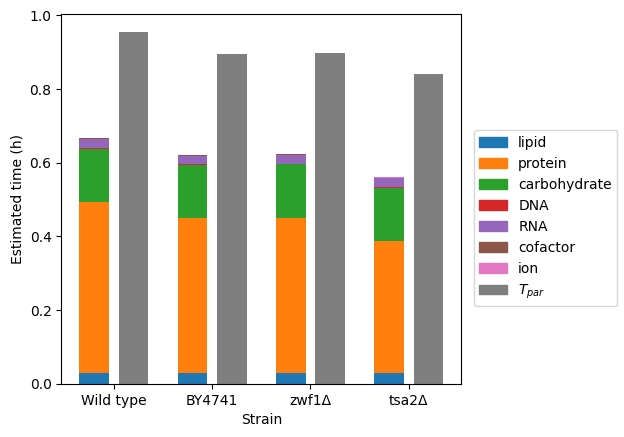
\includegraphics[width=0.7\textwidth]{deletions}

  \caption[
    Estimated synthesis times of biomass components, for BY4741, \textit{zwf$\Delta$}, and \textit{tsa2$\Delta$}
  ]{
    Estimated synthesis times of biomass components: from ablation and $\Tpar$, for wild-type (unmodified model), BY4741, \textit{zwf$\Delta$} in the BY4741 background, and \textit{tsa2$\Delta$} in the BY4742 background
  }
  \label{fig:model-ablation-strains}
\end{figure}


\section{Effect of restricting the enzyme pool}
\label{sec:model-pool}

The yeast cell has a finite enzyme-available proteome pool, so it must decide which enzymes to allocate the greatest proportions of the pool to.
To study this effect using the ecYeast8 model, I imposed a constraint on the enzyme-available proteome pool by varying the value of the upper limit of the flux $\epool$ of the enzyme pool pseudoreaction (Eq.\ \ref{eq:model-gecko-enzyme-pool}), taking advantage of a GECKO formalism that is easy to modify and interpret.
With a smaller $\epool$, the sum of fluxes of enzyme usage pseudoreactions must decrease, and the model must decide which enzyme usage pseudoreactions to allocate a higher flux to, modelling the biological response to a restricted enzyme pool.

Fig.\ \ref{fig:model-pool} shows that constraining the proteome pool available for enzymes leads to a greater advantage of sequential biosynthesis of biomass components over parallel biosynthesis.
Within the range of $\epool^{\prime}$ that gives realistic growth rates, this is evidenced by a decreasing $\ratioabl$ ratio if $\epool^{\prime}$ decreases (Fig.\ \ref{fig:model-pool-ratio-growthrate}).
Concurrently, as $\epool^{\prime}$ decreases, the wild type growth rate ($\gro$) decreases linearly to zero and ablated growth rates ($\griabl$) decrease in linear segments independently of each other and of the growth rate.
These observations can be explained by considering Eq.\ \ref{eq:model-ratio} and modelling the changes of $\gro$ and $\griabl$ with respect to $\epool^{\prime}/\epool$ as linear equations (Appendix~\ref{append:model-pool}).

\begin{figure}[htb!]
  \centering
  \begin{subfigure}[htpb]{0.45\textwidth}
   \centering
   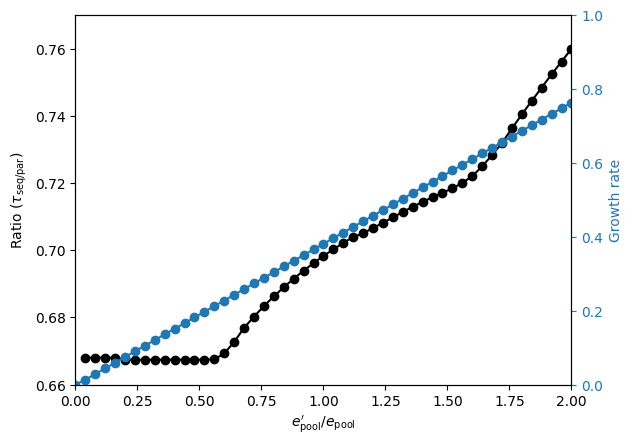
\includegraphics[width=\textwidth]{epool_ec_ratio_gr}
   \caption{
   }
   \label{fig:model-pool-ratio-growthrate}
  \end{subfigure}%
  \begin{subfigure}[htpb]{0.45\textwidth}
   \centering
   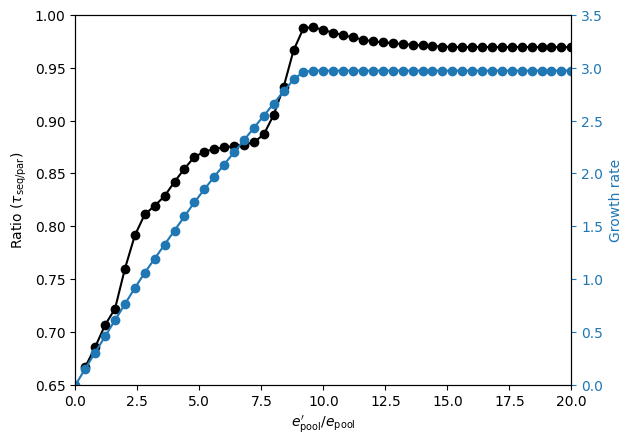
\includegraphics[width=\textwidth]{epool_ec_ratio_gr_20}
   \caption{
   }
   \label{fig:model-pool-ratio-growthrate-20}
  \end{subfigure}

  \begin{subfigure}[htpb]{0.45\textwidth}
   \centering
   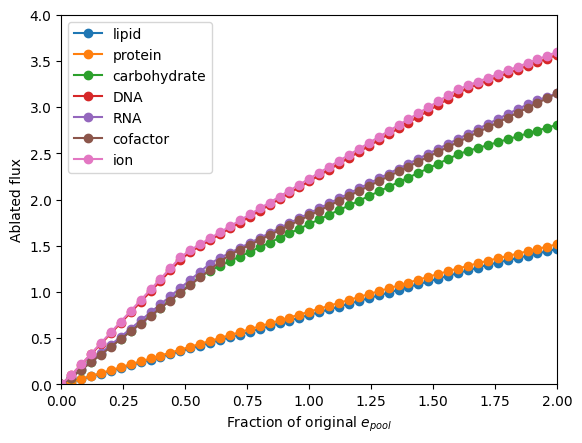
\includegraphics[width=\textwidth]{epool_ec_components}
   \caption{
   }
   \label{fig:model-pool-ablated}
  \end{subfigure}%
  \begin{subfigure}[htpb]{0.45\textwidth}
   \centering
   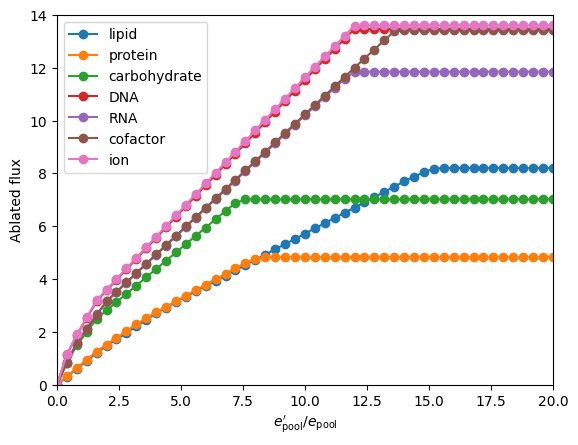
\includegraphics[width=\textwidth]{epool_ec_components_20}
   \caption{
   }
   \label{fig:model-pool-ablated-20}
  \end{subfigure}

  \caption[
    Effect of the size of the proteome pool available for enzymes
  ]{
    Effect of the size of the proteome pool available for enzymes ($\epool^{\prime}$) on \textbf{(\ref{fig:model-pool-ratio-growthrate},~\ref{fig:model-pool-ratio-growthrate-20})} $\ratioabl$, the growth rate, and \textbf{(\ref{fig:model-pool-ablated},~\ref{fig:model-pool-ablated-20})} the optimal flux of the ablated biomass reaction $\griabl$ in each round of ablation.
    \textbf{(\ref{fig:model-pool-ratio-growthrate})} and \textbf{(\ref{fig:model-pool-ablated})} show $\epool^{\prime}/\epool \leq 2$, while
    \textbf{(\ref{fig:model-pool-ratio-growthrate-20})} and \textbf{(\ref{fig:model-pool-ablated-20})} show $\epool^{\prime}/\epool \leq 20$.
  }
  \label{fig:model-pool}
\end{figure}


\section{Effect of carbon and nitrogen sources}
\label{sec:model-exchange}

To explore whether sequential synthesis of biomass components remains advantageous across nutrient conditions, I investigated how changes in the concentrations of nitrogen (ammonium) and carbon sources (glucose and pyruvate) affected the resource allocation strategies.
Ammonium is the form of nitrogen in minimal growth media.
Glucose is the preferred carbon source for budding yeast, and as pyruvate is a non-fermentable carbon source, using it as a carbon source would show how substantial changes to central carbon metabolism affected resource allocation strategies.

\subsection{Saturation of exchange reactions}
\label{subsec:model-saturation}

Investigating the effect of carbon and nitrogen sources requires finding ranges of concentrations of each source to be used in an FBA problem that leads to biologically informative results.
The saturation point of the nutrient, defined as the concentration of the nutrient at which the growth rate reaches its maximum, thus serves as a biologically relevant reference point.
Although genome-scale metabolic models have nutrient exchange reactions that simulate the presence or absence of nutrients, saturation points from experimental studies cannot be directly used as flux bounds for these reactions because FBA does not account for substrate concentrations.
Instead, I constrained the flux of exchange reactions so that the optimised growth rate matched experimental observations, as was performed in previous FBA-based studies \parencite{elsemmanWholecellModelingYeast2022,familiSaccharomycesCerevisiaePhenotypes2003}.

To model the effect of nutrient concentrations on growth rate, I created saturation curves that show how the effect of nutrient exchange flux on the objective function.
%These curves were created by varying the upper bounds of nutrient exchange reactions and optimising the model at each upper bound value.
Figs.\ \ref{fig:model-saturation-glucose} and~\ref{fig:model-saturation-pyruvate} show that the saturation curves of glucose and pyruvate had different shapes.
In addition, the maximum growth rate on glucose (\SI{0.38}{\hour^{-1}}) was greater than the maximum growth rate on pyruvate (\SI{0.25}{\hour^{-1}}).
Furthermore, Fig.\ \ref{fig:model-saturation-ammonium} shows that the maximum growth rate on the carbon source sets the saturation point for ammonium.

\begin{figure}[hbp!]
  \centering
  \begin{subfigure}[t]{0.45\textwidth}
  \centering
    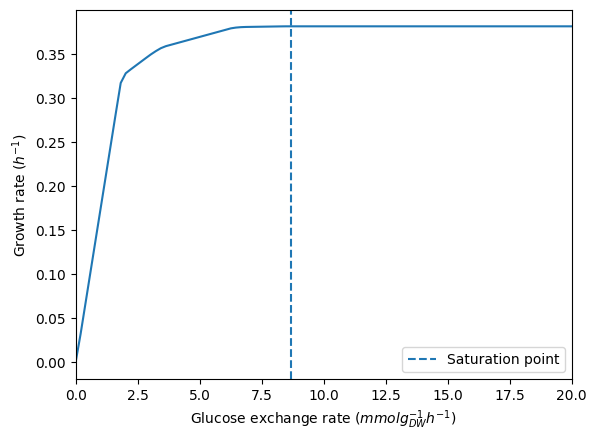
\includegraphics[width=\linewidth]{saturation_glc}
    \caption{
      % Effect of glucose exchange on growth rate, with ammonium exchange flux unrestricted.
      % Growth rate saturation is at \SI{8.69}{\mmolgdwh}.
    }
    \label{fig:model-saturation-glucose}
  \end{subfigure}%
  \begin{subfigure}[t]{0.45\textwidth}
  \centering
    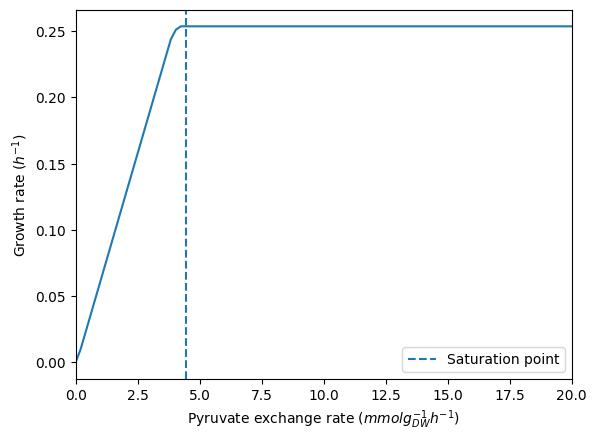
\includegraphics[width=\linewidth]{saturation_pyr}
    \caption{
      % Effect of pyruvate exchange on growth rate, with ammonium exchange flux unrestricted.
      % Growth rate saturation is at \SI{4.44}{\mmolgdwh}.
    }
    \label{fig:model-saturation-pyruvate}
  \end{subfigure}

  \begin{subfigure}[t]{0.45\textwidth}
  \centering
    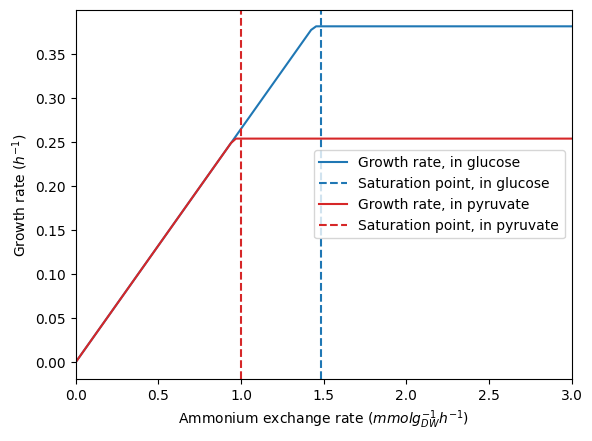
\includegraphics[width=\linewidth]{saturation_amm}
    \caption{
      % Effect of ammonium exchange on growth rate, with exchanges of carbon sources set to growth rate saturation based on figures~\ref{fig:model-saturation-glucose} and ~\ref{fig:model-saturation-pyruvate}.
      % Growth rate saturation is at \SI{1.48}{\mmolgdwh} in glucose, and
      % at \SI{1.00}{\mmolgdwh} in pyruvate.
    }
    \label{fig:model-saturation-ammonium}
  \end{subfigure}

  \caption[
    Effect of exchange reactions on growth rate
  ]{
    Effect of glucose \textbf{(\ref{fig:model-saturation-glucose})}, pyruvate \textbf{(\ref{fig:model-saturation-pyruvate})}, and ammonium \textbf{(\ref{fig:model-saturation-ammonium})} exchange reactions on growth rate.
    The saturation point of exchange reactions is defined as the flux of an exchange reaction above which the objective function reaches its maximum.
  }
  \label{fig:model-saturation}
\end{figure}

These growth saturation curves agree with similar studies.
Specifically, the growth saturation curve for glucose (Fig.\ \ref{fig:model-saturation-glucose}) is similar to that simulated by \textcite{elsemmanWholecellModelingYeast2022} using another derivative of the Yeast8 model.
The maximum growth rate on glucose agrees with \textcite{domenzainReconstructionCatalogueGenomescale2022}, which used GECKO 2 to create the ecYeast7 model to predict maximum growth rates on various carbon sources.
\textcite{domenzainReconstructionCatalogueGenomescale2022} did not simulate growth on pyruvate, but a lower maximum growth rate on pyruvate is consistent with my experimental observations.


\subsection{Effect of carbon and nitrogen sources on biomass synthesis strategies}
\label{subsec:model-grid}

\subsubsection{Glucose and ammonium}
\label{subsec:model-grid-glucose}

% To visualise the extent to which each exchange rate limits each quantity of interest, I show the sensitivity values as arrows (Figs.\ \ref{fig:model-grid-glc} and~\ref{fig:model-grid-pyr}) with $s_{\mathrm{glc}}$ and $s_{\mathrm{amm}}$ as two components of the vector that defines these arrows.
% Thus, horizontal arrows indicate a strong sensitivity to glucose and vertical arrows indicate a strong sensitivity to ammonium, while the arrows point towards increasing values of the quantity of interest.

To assess the effect of glucose and ammonium concentration on biomass synthesis strategies, I ablated components in the biomass reaction in different nutrient conditions set by glucose and ammonium exchange fluxes
to obtain $\ratioabl$, $\gro$, $\Tabl{carbohydrate}$, and $\Tabl{protein}$.
Additionally, to determine whether the carbon or nitrogen source is limiting for each of these quantities, I defined the sensitivity at each nutrient condition $(\exchrate{glc}, \exchrate{amm})$, with respect to each axis $i$ as:

\begin{equation}
  s_{i}(\exchrate{glc}, \exchrate{amm}) = \frac{R_{i}}{y(\exchrate{glc}, \exchrate{amm})} \cdot \pdif{y(\exchrate{glc}, \exchrate{amm})}{R_{i}}
  \label{eq:model-susceptibility}
\end{equation}

where
$i$ indicates glucose (glc) or ammonium (amm),
$R_{i}$ indicates the exchange rate, glucose ($\exchrate{glc}$) or ammonium ($\exchrate{amm}$),
an $(\exchrate{glc}, \exchrate{amm})$ pair defines a nutrient condition, and
$y(\exchrate{glc}, \exchrate{amm})$ represents the quantity of interest at each nutrient condition.
For a specific nutrient condition $(\exchrate{glc}, \exchrate{amm})$, if $s_{\mathrm{glc}}(\exchrate{glc}, \exchrate{amm}) > s_{\mathrm{amm}}(\exchrate{glc}, \exchrate{amm})$ for a quantity of interest $y$, then the quantity is more sensitive to glucose exchange in this condition.
Conversely, if $s_{\mathrm{glc}}(\exchrate{glc}, \exchrate{amm}) < s_{\mathrm{amm}}(\exchrate{glc}, \exchrate{amm})$, the quantity is more sensitive to ammonium exchange.

Fig.\ \ref{fig:model-grid-glc-growthrate} divides the nutrient conditions into three regions according to nutrient limitation: a glucose-limiting region, an ammonium-limiting region, and a region where neither glucose nor ammonium is limiting.
These regions are determined by $(s_{\mathrm{glc}}, s_{\mathrm{amm}})$ vectors.
Fig.\ \ref{fig:model-grid-glc-ratio} shows that parallel biosynthesis was advantageous ($\ratioabl > 1$) in two circumstances: when both glucose and ammonium limited the growth rate, and when ammonium exchange was at saturation while glucose exchange is greater than saturation.
In contrast, when the growth rate was near its maximum, where neither glucose nor ammonium was limiting, when glucose or ammonium exchange increased, sequential biosynthesis became more advantageous ($\ratioabl < 1$).

\begin{figure}
  \centering
  \begin{subfigure}[t]{0.45\textwidth}
  \centering
    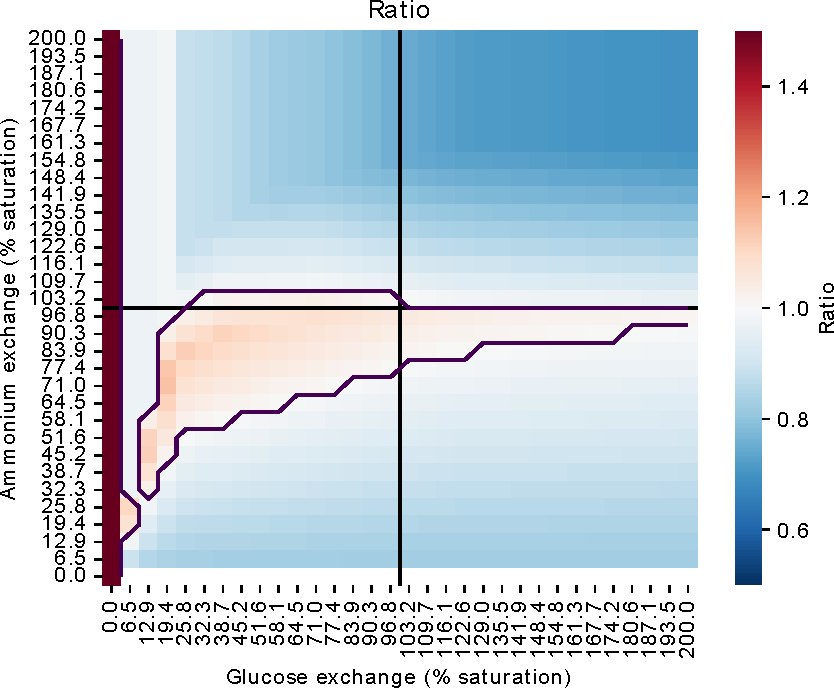
\includegraphics[width=\linewidth]{ec_grid_glc_amm_ratio}
    \caption{
    }
    \label{fig:model-grid-glc-ratio}
  \end{subfigure}%
  \begin{subfigure}[t]{0.45\textwidth}
  \centering
    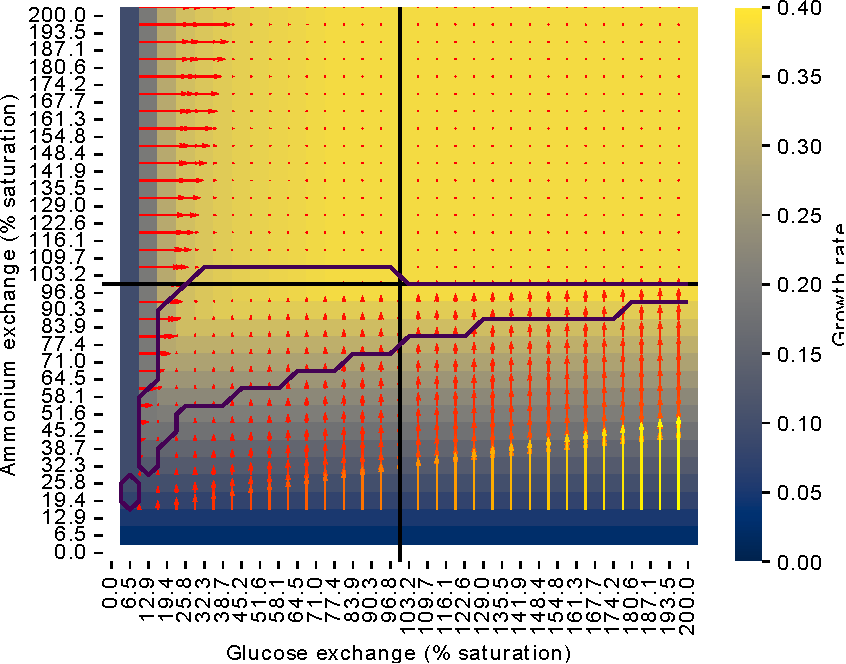
\includegraphics[width=\linewidth]{ec_grid_glc_amm_gr}
    \caption{
    }
    \label{fig:model-grid-glc-growthrate}
  \end{subfigure}

  \begin{subfigure}[t]{0.45\textwidth}
  \centering
    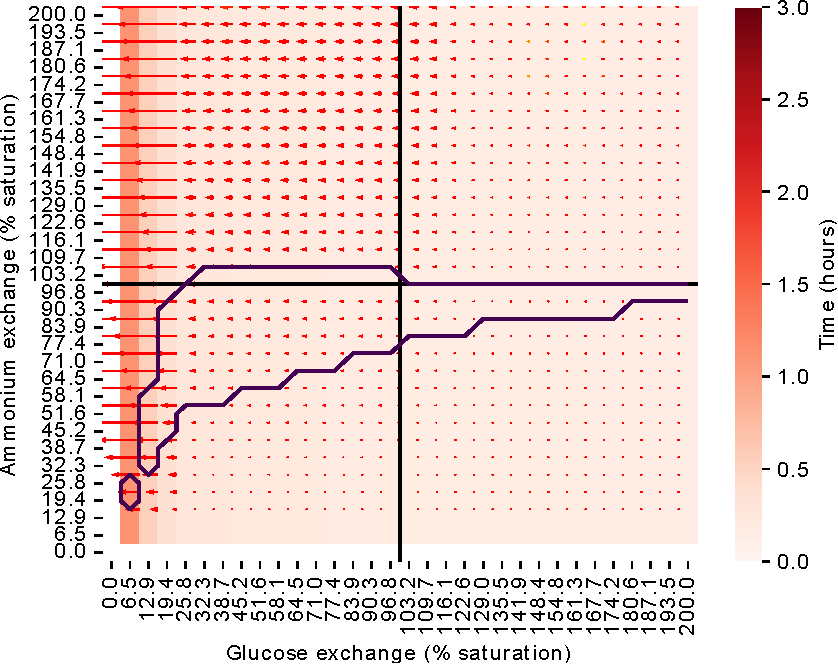
\includegraphics[width=\linewidth]{ec_grid_glc_amm_carb}
    \caption{
    }
    \label{fig:model-grid-glc-carb}
  \end{subfigure}%
  \begin{subfigure}[t]{0.45\textwidth}
  \centering
    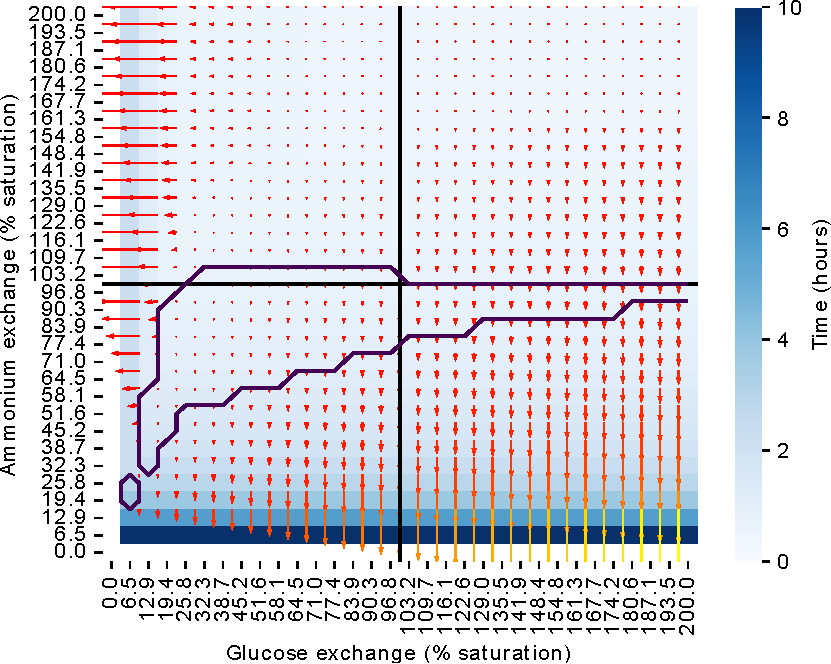
\includegraphics[width=\linewidth]{ec_grid_glc_amm_prot}
    \caption{
    }
    \label{fig:model-grid-glc-prot}
  \end{subfigure}

  \begin{subfigure}[t]{0.45\textwidth}
  \centering
    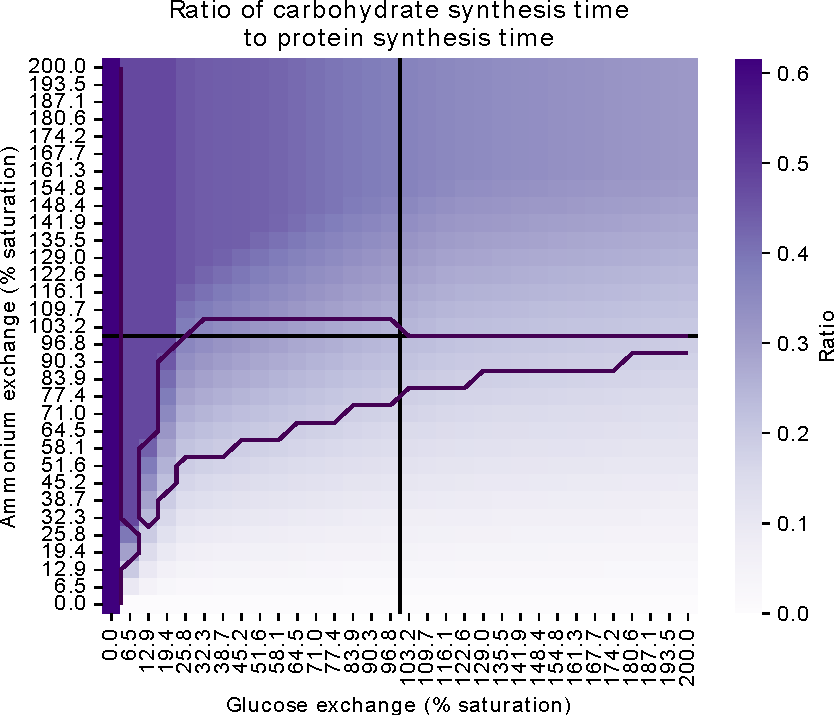
\includegraphics[width=\linewidth]{ec_grid_glc_amm_carb_to_prot}
    \caption{
    }
    \label{fig:model-grid-glc-carb-to-prot}
  \end{subfigure}
  \caption[
    Effect of glucose and ammonium exchange rates
  ]{
    Effect of glucose and ammonium exchange rates on \textbf{(\ref{fig:model-grid-glc-ratio})} $\ratioabl$, \textbf{(\ref{fig:model-grid-glc-growthrate})} growth rate based on unmodified biomass reaction, $\gro$, \textbf{(\ref{fig:model-grid-glc-carb})} predicted carbohydrate synthesis time, $\Tabl{carbohydrate}$ \textbf{(\ref{fig:model-grid-glc-prot})} predicted protein synthesis time, $\Tabl{protein}$, and \textbf{(\ref{fig:model-grid-glc-carb-to-prot})} ratio of carbohydrate synthesis time to protein synthesis time, $\Tabl{carbohydrate}/\Tabl{protein}$.
    Exchange rates are expressed in percentages of growth saturation from Fig.\ \ref{fig:model-saturation}, with black straight lines indicate 100\% of saturation.
    Contours show regions in which $\ratioabl > 1$.
    Arrows overlaid on heatmaps indicate sensitivity of the quantity as a vector $(s_{\mathrm{glc}}, s_{\mathrm{amm}})$ (Eq.\ \ref{eq:model-susceptibility}).
  }
  \label{fig:model-grid-glc}
\end{figure}

To link the changes in the values of $\Tabl{carbohydrate}$ and $\Tabl{protein}$ with cellular biochemistry, Fig.\ \ref{fig:model-grid-glc-carb} and~\ref{fig:model-grid-glc-prot} show how both values are affected by $\exchrate{glc}$ and $\exchrate{amm}$.
Fig.\ \ref{fig:model-grid-glc-carb} shows that glucose exchange limited carbohydrate synthesis time in all nutrient conditions, and this observation could be explained by glucose uptake being directly linked to carbohydrate synthesis.
In contrast, Fig.\ \ref{fig:model-grid-glc-prot} shows that ammonium exchange limited protein synthesis time for most nutrient conditions, except for conditions in which glucose exchange was very low.
This observation can be explained by the fact that both carbon and nitrogen sources contribute to protein biosynthesis.

To determine whether changes in the synthesis time of biomass components are responsible for switching of scheduling strategies between sequential and parallel biosynthesis, I investigated how $\exchrate{glc}$ and $\exchrate{amm}$ affected $\frac{\Tabl{carbohydrate}}{\Tabl{protein}}$.
Synthesis times $\Tiabl$ were computed to assess whether the ratio between the synthesis times differed in different conditions.
The ratio $\frac{\Tabl{carbohydrate}}{\Tabl{protein}}$ serves as the principal measure to quantify how $\Tiabl$ values change as nutrient conditions change.
This ratio is informative because:
\begin{enumerate}
  \item Of all biomass components, predicted synthesis times of these biomass components varied the most as the glucose and ammonium exchange rates were varied.
  \item Each accounts for a large proportion of biomass: protein accounts for 52.5\% and carbohydrate accounts for 36.4\% (Table~\ref{tab:model-biomfrac}).
  \item Carbohydrate synthesis has a clear biochemical relationship with the level of a carbon source.
        Additionally, protein synthesis has a clear biochemical relationship with the level of ammonium as amino acids contain amino groups.
\end{enumerate}

% Based on equation~\ref{eq:model-ablated-time}, consider:

% \begin{equation}
%   \frac{\Tabl{carbohydrate}}{\Tabl{protein}} = \frac{\biomfrac{carbohydrate}}{\biomfrac{protein}} \cdot \frac{\grabl{protein}}{\grabl{carbohydrate}}
%   \label{eq:model-carb-prot-ratio}
% \end{equation}

Fig.\ \ref{fig:model-grid-glc-carb-to-prot} suggests that carbon and nitrogen limitation affect the ratios of synthesis times among biomass components, as shown by the change in the value of $\frac{\Tabl{carbohydrate}}{\Tabl{protein}}$ as $\exchrate{glc}$ and $\exchrate{amm}$ changed.
Specifically, within the glucose-limiting region, $\frac{\Tabl{carbohydrate}}{\Tabl{protein}}$ was at a high and constant value.
In contrast, within the ammonium-limiting region, as $\exchrate{amm}$ increases, $\frac{\Tabl{carbohydrate}}{\Tabl{protein}}$ increased.
In addition, along the boundary of both regions, where glucose and ammonium were both near-limiting and $\ratioabl$ was high, $\frac{\Tabl{carbohydrate}}{\Tabl{protein}}$ remained roughly constant.
These observations link synthesis times of biomass components with scheduling strategy.
Specifically, the observations suggest that the ratios of synthesis times alone did not explain the choice of scheduling strategy, and that total biosynthesis time was an additional factor.

\subsubsection{Pyruvate and ammonium}
\label{subsec:model-grid-pyruvate}

To investigate the effect of a non-fermentable carbon source on biomass synthesis strategies, I repeated the investigation using pyruvate as the carbon source. %, ablating components in the biomass reaction in different nutrient conditions.%, and adjusted the saturation exchange rates accordingly: pyruvate saturation being at \SI{4.44}{\mmolgdwh} and ammonium saturation being at \SI{1.00}{\mmolgdwh} (figure~\ref{fig:model-grid-pyr}).

Results show that the saturation curve of pyruvate controlled the effect of exchange rates on scheduling strategies.
Fig.\ \ref{fig:model-grid-pyr} shows that when pyruvate was the carbon source, the region of carbon source limitation was larger than when glucose was the carbon source.
This observation reflected the different shapes of the pyruvate and glucose saturation curves (Fig.\ \ref{fig:model-saturation}): on glucose, the growth rate reached half of its maximum value when glucose exchange was well below half saturation, while on pyruvate the growth rate reached half of its maximum value when pyruvate exchange was half saturation.

\begin{figure}
  \centering
  \begin{subfigure}[t]{0.45\textwidth}
  \centering
    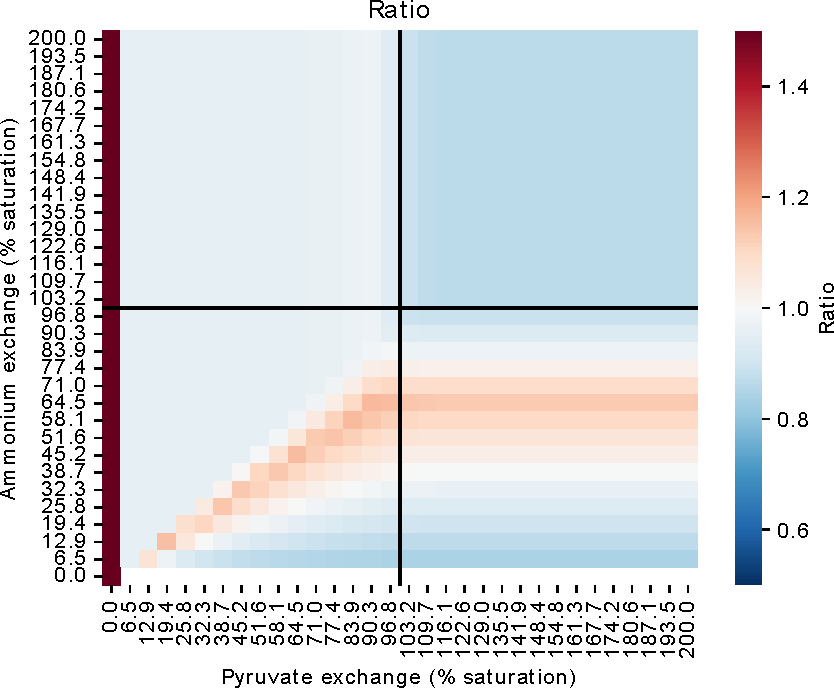
\includegraphics[width=\linewidth]{ec_grid_pyr_amm_ratio}
    \caption{
    }
    \label{fig:model-grid-pyr-ratio}
  \end{subfigure}%
  \begin{subfigure}[t]{0.45\textwidth}
  \centering
    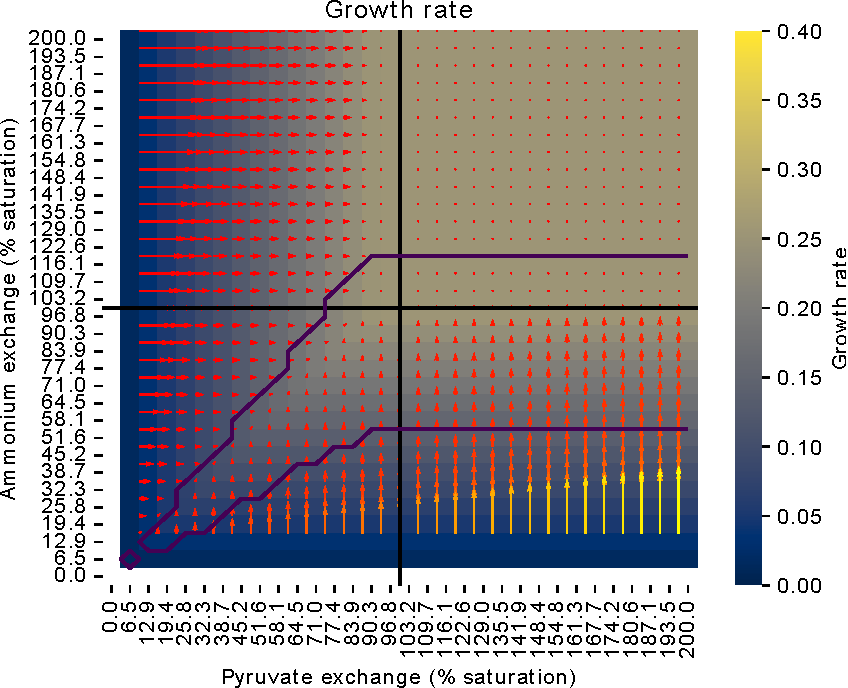
\includegraphics[width=\linewidth]{ec_grid_pyr_amm_gr}
    \caption{
    }
    \label{fig:model-grid-pyr-growthrate}
  \end{subfigure}

  \begin{subfigure}[t]{0.45\textwidth}
  \centering
    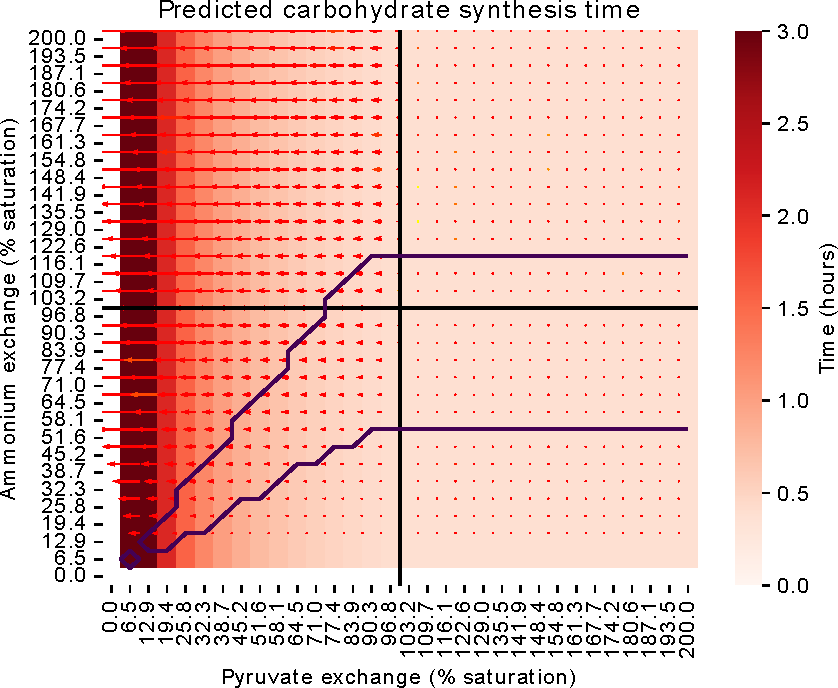
\includegraphics[width=\linewidth]{ec_grid_pyr_amm_carb}
    \caption{
    }
    \label{fig:model-grid-pyr-carb}
  \end{subfigure}%
  \begin{subfigure}[t]{0.45\textwidth}
  \centering
    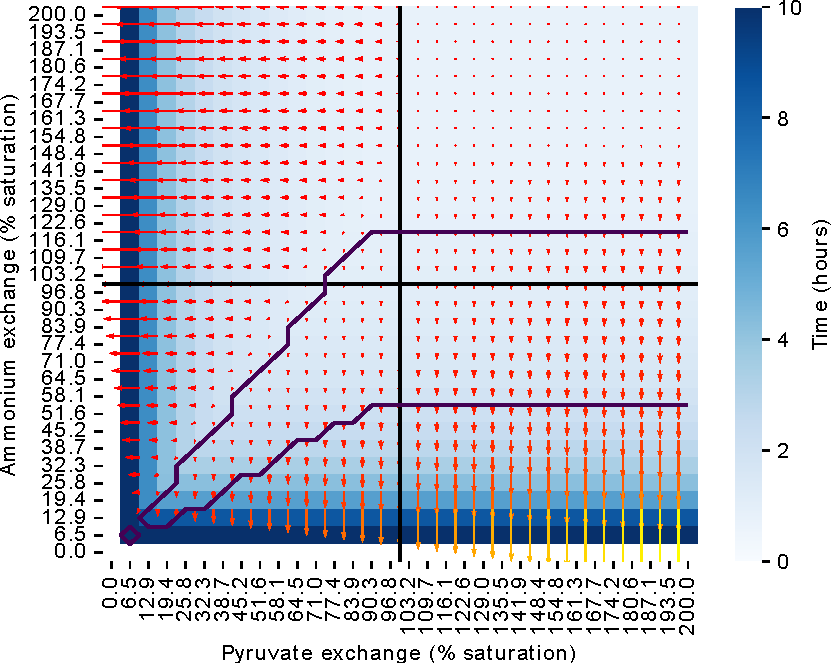
\includegraphics[width=\linewidth]{ec_grid_pyr_amm_prot}
    \caption{
    }
    \label{fig:model-grid-pyr-prot}
  \end{subfigure}

  \begin{subfigure}[t]{0.45\textwidth}
  \centering
    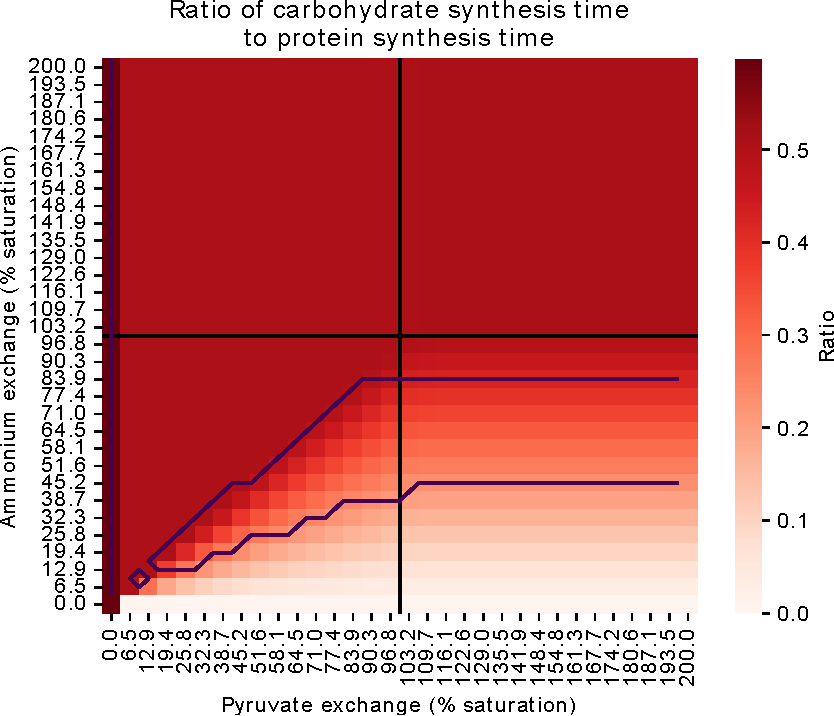
\includegraphics[width=\linewidth]{ec_grid_pyr_amm_carb_to_prot}
    \caption{
    }
    \label{fig:model-grid-pyr-carb-to-prot}
  \end{subfigure}
  \caption[
    Effect of pyruvate and ammonium exchange rates
  ]{
    Effect of pyruvate and ammonium exchange rates on \textbf{(\ref{fig:model-grid-pyr-ratio})} $\ratioabl$, \textbf{(\ref{fig:model-grid-pyr-growthrate})} growth rate based on unmodified biomass reaction, $\gro$, \textbf{(\ref{fig:model-grid-pyr-carb})} predicted carbohydrate synthesis time, $\Tabl{carbohydrate}$ \textbf{(\ref{fig:model-grid-pyr-prot})} predicted protein synthesis time, $\Tabl{protein}$, and \textbf{(\ref{fig:model-grid-pyr-carb-to-prot})} ratio of carbohydrate synthesis time to protein synthesis time, $\Tabl{carbohydrate}/\Tabl{protein}$.
    Exchange rates are expressed in percentages of growth saturation from Fig.\ \ref{fig:model-saturation}, with black straight lines indicate 100\% of saturation.
    Contours show regions in which $\ratioabl > 1$.
    Arrows overlaid on heatmaps indicate sensitivity of the quantity as a vector $(s_{\mathrm{pyr}}, s_{\mathrm{amm}})$ (Eq.\ \ref{eq:model-susceptibility}).
  }
  \label{fig:model-grid-pyr}
\end{figure}

Fig.\ \ref{fig:model-grid-pyr} shows that the relationships between exchange rates and the quantities $\ratioabl$, $\gro$, $\Tabl{carbohydrate}$, and $\Tabl{protein}$ were similar to the glucose-ammonium case.
In other words, when pyruvate was the carbon source, the relationship between carbon and nitrogen source uptake and the synthesis of carbohydrates and proteins still determined how scheduling strategies changed according to nutrient conditions.
Parallel biosynthesis was advantageous in two conditions: when both pyruvate and ammonium limited the growth rate, and when ammonium exchange was at saturation while pyruvate exchange was greater than saturation (Fig.\ \ref{fig:model-grid-pyr-ratio}).
In contrast, sequential biosynthesis was advantageous when neither pyruvate nor ammonium was limiting.
$\frac{\Tabl{carbohydrate}}{\Tabl{protein}}$ remained at high values when pyruvate is limiting or when pyruvate and ammonium were both limiting (Fig.\ \ref{fig:model-grid-pyr-carb-to-prot}).
Furthermore, the behaviour of $\frac{\Tabl{carbohydrate}}{\Tabl{protein}}$ as nutrient conditions varied could also be explained by pyruvate exchange limiting carbohydrate synthesis time (Fig.\ \ref{fig:model-grid-pyr-carb}) and by both pyruvate and ammonium exchange limiting protein synthesis time (Fig.\ \ref{fig:model-grid-pyr-prot}).


\subsection{Relationship between proteome allocation and resource allocation strategy}
\label{subsec:model-rank}

\subsubsection{Glucose and ammonium}
\label{subsec:model-rank-glucose}

The investigation of the effect of carbon and nitrogen sources on scheduling strategies led to a new hypothesis: the cell favours parallel biosynthesis of biomass components when the carbon source and the nitrogen source are both limiting, especially if the associated biomass components share metabolic pathways and if the conditions dictate similar levels of enzymes.
This hypothesis arose from the observation that the highest $\ratioabl$ occurred at the boundary at which both the carbon source and the nitrogen source were limiting.

To evaluate this hypothesis, I compared the enzyme usage reaction flux vectors in rounds of ablation between a high $\ratioabl$ condition and a low $\ratioabl$ condition created by combinations of glucose and ammonium exchange rates.
Enzyme usage reaction flux vectors show how the cell allocates its finite proteome to enzymes when each biomass component is prioritised (Section~\ref{sec:model-timescale}).

To test whether similarities in proteome allocation to enzymes explain parallel biosynthesis, Fig.\ \ref{fig:model-rank-glc-highratio-rank} shows that when both glucose and ammonium were limiting, the allocation patterns were similar across rounds of ablation, thus explaining the advantage of parallel biosynthesis of biomass components.
This similarity is quantified in Fig.\ \ref{fig:model-rank-glc-highratio-kendall}, which shows that parallel biosynthesis exhibited relatively similar proteome allocation with the synthesis of individual biomass components.

\begin{figure}[htbp!]
  \centering
  \begin{subfigure}[t]{0.45\textwidth}
  \centering
    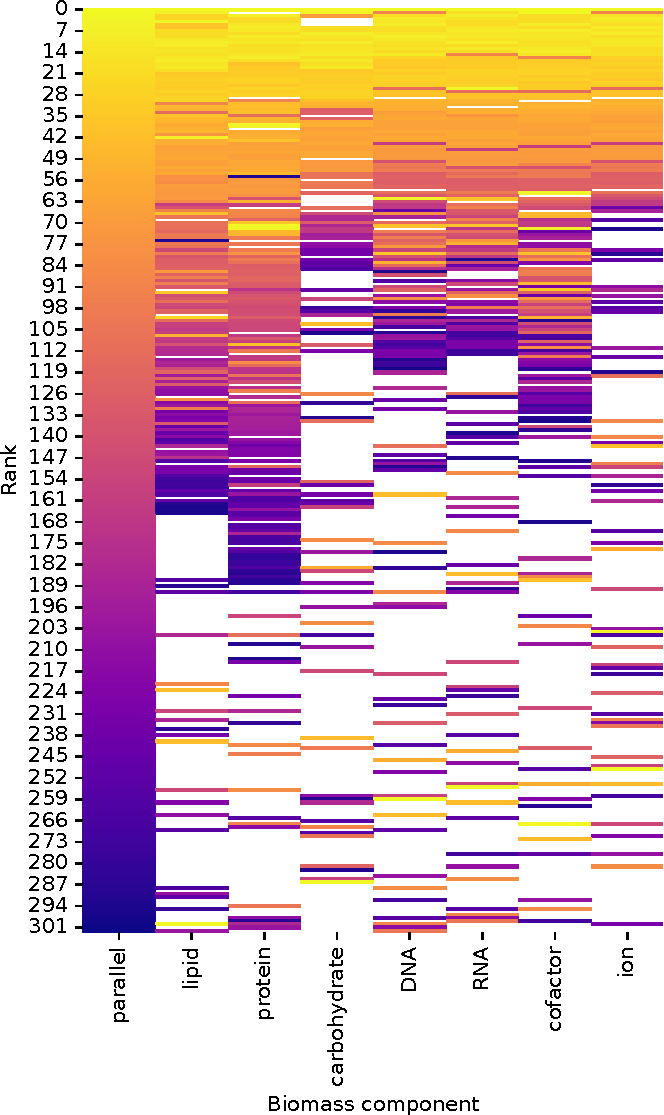
\includegraphics[width=\linewidth]{CompareEnzUse_glc01p69_pyrUnres_amm01p05_1.pdf}
    \caption{
    }
    \label{fig:model-rank-glc-highratio-rank}
  \end{subfigure}%
  \begin{subfigure}[t]{0.45\textwidth}
  \centering
    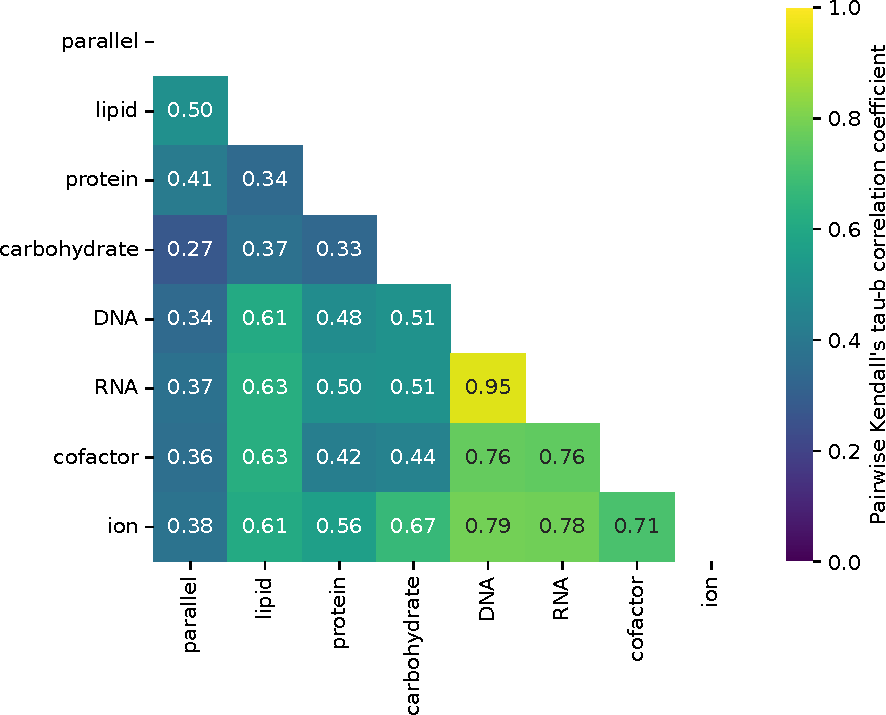
\includegraphics[width=\linewidth]{CompareEnzUse_glc01p69_pyrUnres_amm01p05_2.pdf}
    \caption{
    }
    \label{fig:model-rank-glc-highratio-kendall}
  \end{subfigure}%

  \caption[
    Changes in enzyme usage reaction flux and Kendall's $\tau$-b rank correlation coefficient for each pair, $\exchrate{glc}$ = \SI{1.69}{\mmolgdwh}, $\exchrate{amm}$ = \SI{1.05}{\mmolgdwh}.
    ]{
    For the high $\ratioabl$ condition ($\exchrate{glc}$ = \SI{1.69}{\mmolgdwh}, $\exchrate{amm}$ = \SI{1.05}{\mmolgdwh}):
    \textbf{(\ref{fig:model-rank-glc-highratio-rank})}
    changes in enzyme usage reaction flux in rounds of ablation.
    Columns show the biomass component prioritised.
    In each column, rows represent enzyme usage reactions, arranged in descending order of flux.
    Colours identify the reactions, with white indicating reactions that carry zero flux in the parallel case.
    \textbf{(\ref{fig:model-rank-glc-highratio-kendall})}
    Pairwise Kendall's $\tau$-b rank correlation coefficient \parencite{kendallTREATMENTTIESRANKING1945} for each pair of enzyme usage flux profiles.
  }
  \label{fig:model-rank-glc-highratio}
\end{figure}

In contrast, Fig.\ \ref{fig:model-rank-glc-lowratio-rank} shows that when neither glucose nor ammonium limited growth, biomass components could be divided into two groups based on enzyme usage reaction flux vectors.
These groups suggest an explanation for sequential biosynthesis: the cell may synthesise lipids and proteins together in one stage of its growth cycle, while synthesising carbohydrates, DNA, RNA, cofactors, and ions together in another stage.
The bias towards sequential biosynthesis is further emphasised by Fig.\ \ref{fig:model-rank-glc-lowratio-kendall}, which shows that parallel biosynthesis exhibited different proteome allocation compared to the synthesis of individual biomass components.

\begin{figure}
  \centering
  \begin{subfigure}[t]{0.45\textwidth}
  \centering
    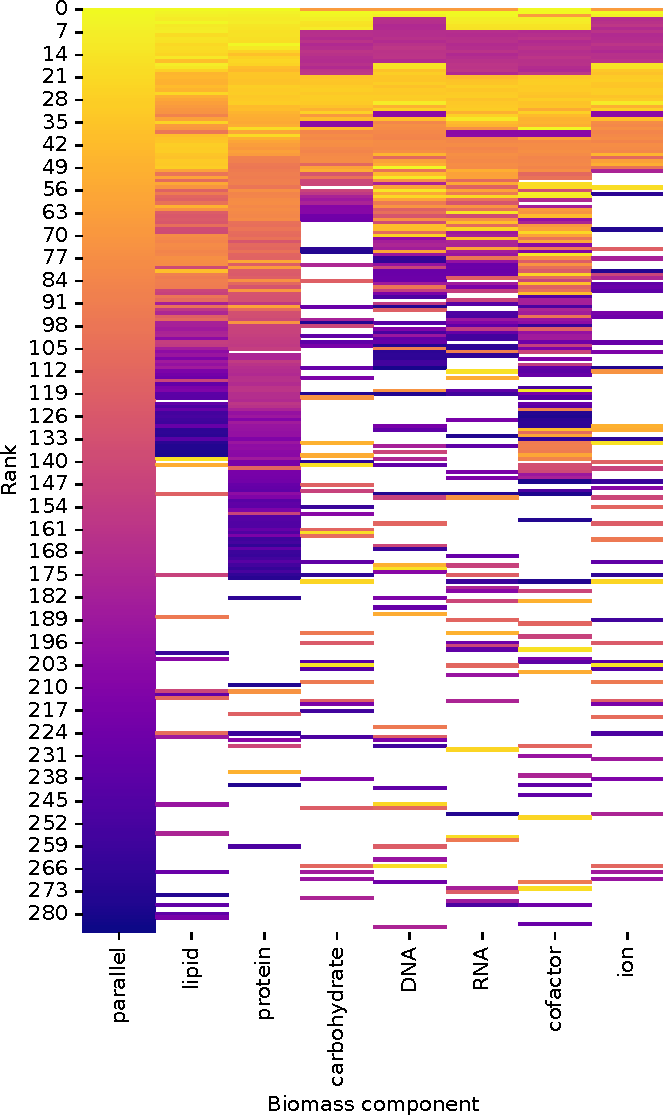
\includegraphics[width=\linewidth]{CompareEnzUse_glc16p89_pyrUnres_ammUnres_1.pdf}
    \caption{
    }
    \label{fig:model-rank-glc-lowratio-rank}
  \end{subfigure}%
  \begin{subfigure}[t]{0.45\textwidth}
  \centering
    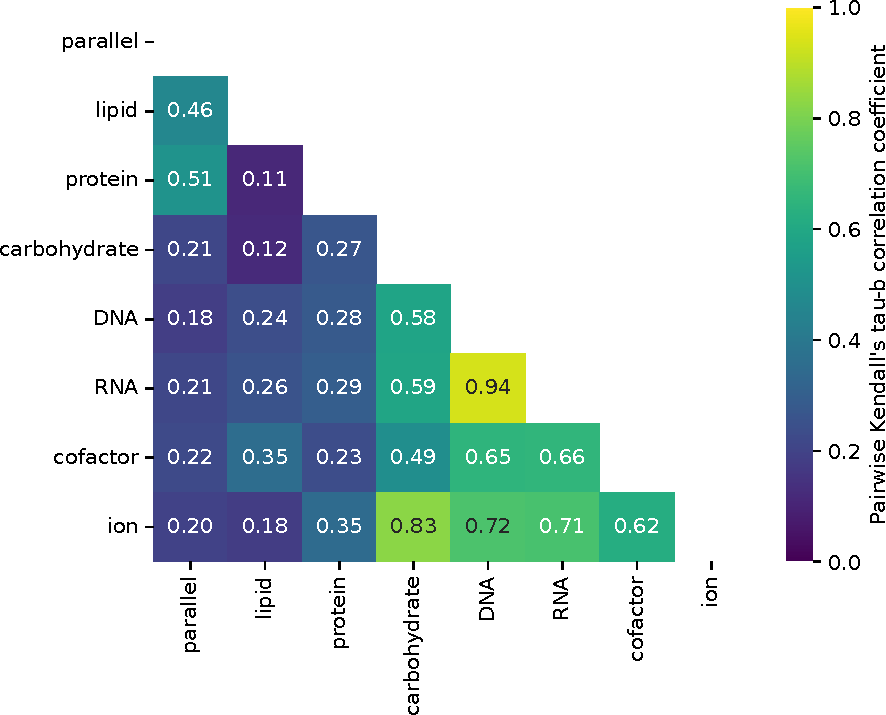
\includegraphics[width=\linewidth]{CompareEnzUse_glc16p89_pyrUnres_ammUnres_2.pdf}
    \caption{
    }
    \label{fig:model-rank-glc-lowratio-kendall}
  \end{subfigure}

  \caption[
    Changes in enzyme usage reaction flux and Kendall's $\tau$-b rank correlation coefficient for each pair, $\exchrate{glc}$ = \SI{16.89}{\mmolgdwh}.
  ]{
    For the low $\ratioabl$ condition ($\exchrate{glc}$ = \SI{16.89}{\mmolgdwh}):
    \textbf{(\ref{fig:model-rank-glc-lowratio-rank})}
    changes in enzyme usage reaction flux in rounds of ablation.
    Columns show the biomass component prioritised.
    In each column, rows represent enzyme usage reactions, arranged in descending order of flux.
    Colours identify the reactions, with white indicating reactions that carry zero flux in the parallel case.
    \textbf{(\ref{fig:model-rank-glc-lowratio-kendall})}
    Pairwise Kendall's $\tau$-b rank correlation coefficient \parencite{kendallTREATMENTTIESRANKING1945} for each pair of enzyme usage flux profiles.
  }
  \label{fig:model-rank-glc-lowratio}
\end{figure}

\pagebreak

\subsubsection{Pyruvate and ammonium}
\label{subsec:model-rank-pyruvate}

To evaluate, in a different carbon source, whether parallel biosynthesis is also favoured when biomass components share metabolic pathways, I extended the comparison of enzyme usage reaction flux vectors in rounds of ablation to nutrient conditions created by pyruvate and ammonium exchange rates.

Similar to the glucose-ammonium investigation, in the high $\ratioabl$ condition where pyruvate and ammonium were limiting, Figs.\ \ref{fig:model-rank-pyr-highratio-rank} and~\ref{fig:model-rank-pyr-highratio-kendall} show that proteome allocation were similar across rounds of ablation, supporting parallel biosynthesis as a scheduling strategy.
However, the results for the low $\ratioabl$ case suggest that grouping of biomass components explains sequential biosynthesis for only very low $\ratioabl$.

\begin{figure}[htbp!]
  \centering
  \begin{subfigure}[t]{0.45\textwidth}
  \centering
    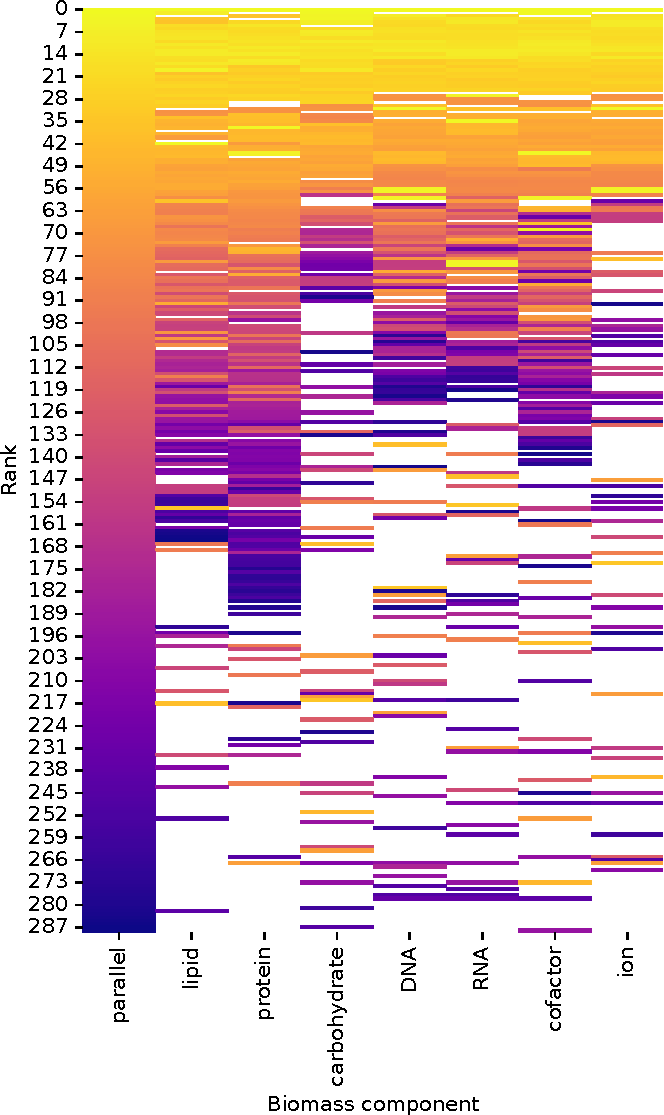
\includegraphics[width=\linewidth]{CompareEnzUse_glc00p00_pyr03p73_amm00p90_1.pdf}
    \caption{
    }
    \label{fig:model-rank-pyr-highratio-rank}
  \end{subfigure}%
  \begin{subfigure}[t]{0.45\textwidth}
  \centering
    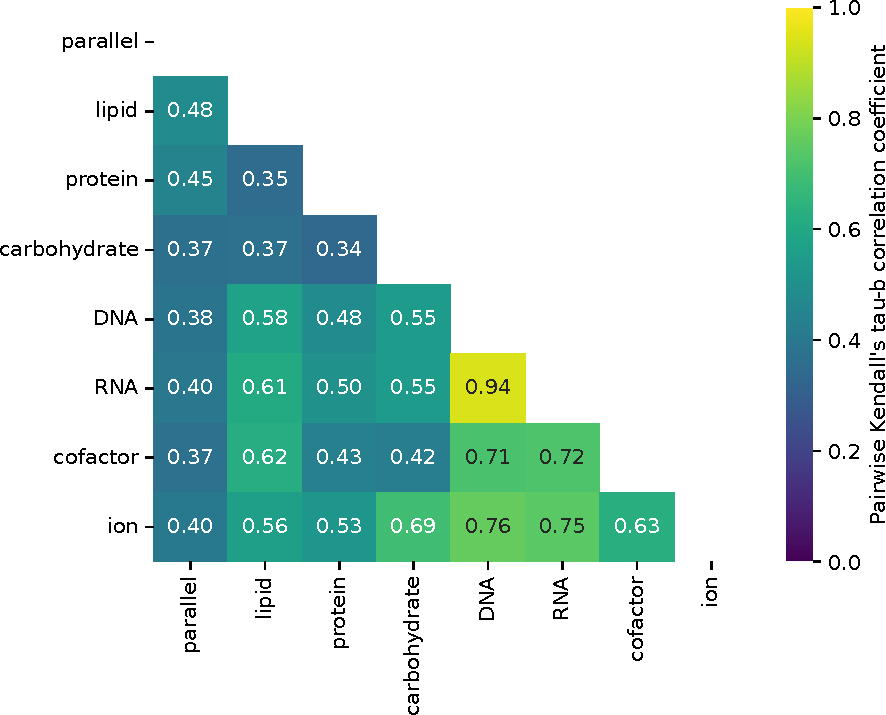
\includegraphics[width=\linewidth]{CompareEnzUse_glc00p00_pyr03p73_amm00p90_2.pdf}
    \caption{
    }
    \label{fig:model-rank-pyr-highratio-kendall}
  \end{subfigure}

  \caption[
    Changes in enzyme usage reaction flux and Kendall's $\tau$-b rank correlation coefficient for each pair, $\exchrate{pyr}$ = \SI{3.73}{\mmolgdwh}, $\exchrate{amm}$ = \SI{0.90}{\mmolgdwh}.
  ]{
    For the high $\ratioabl$ condition ($\exchrate{pyr}$ = \SI{3.73}{\mmolgdwh}, $\exchrate{amm}$ = \SI{0.90}{\mmolgdwh}):
    \textbf{(\ref{fig:model-rank-pyr-highratio-rank})}
    changes in enzyme usage reaction flux in rounds of ablation.
    Columns show the biomass component prioritised.
    In each column, rows represent enzyme usage reactions, arranged in descending order of flux.
    Colours identify the reactions, with white indicating reactions that carry zero flux in the parallel case.
    \textbf{(\ref{fig:model-rank-pyr-highratio-kendall})}
    Pairwise Kendall's $\tau$-b rank correlation coefficient \parencite{kendallTREATMENTTIESRANKING1945} for each pair of enzyme usage flux profiles.
  }
  \label{fig:model-rank-pyr-highratio}
\end{figure}

Fig.\ \ref{fig:model-rank-pyr-lowratio-rank} shows that when pyruvate was the carbon source, the contrast of proteome allocation between biomass components in the low $\ratioabl$ condition was lessened compared to when glucose was the carbon source.
This may be explained by the higher $\ratioabl$ in this condition ($\ratioabl = 0.9$), compared to the $\ratioabl$ in the glucose-ammonium investigation ($\ratioabl = 0.7$).

\begin{figure}[htbp!]
  \centering
  \begin{subfigure}[t]{0.45\textwidth}
  \centering
    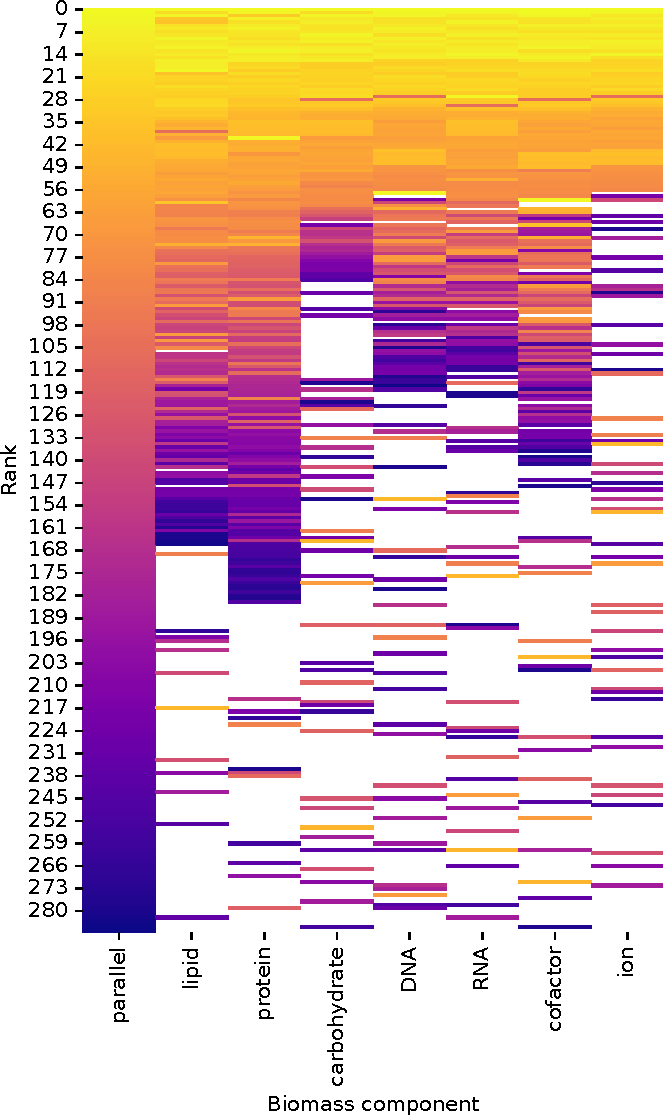
\includegraphics[width=\linewidth]{CompareEnzUse_glc00p00_pyr08p89_ammUnres_1.pdf}
    \caption{
    }
    \label{fig:model-rank-pyr-lowratio-rank}
  \end{subfigure}%
  \begin{subfigure}[t]{0.45\textwidth}
  \centering
    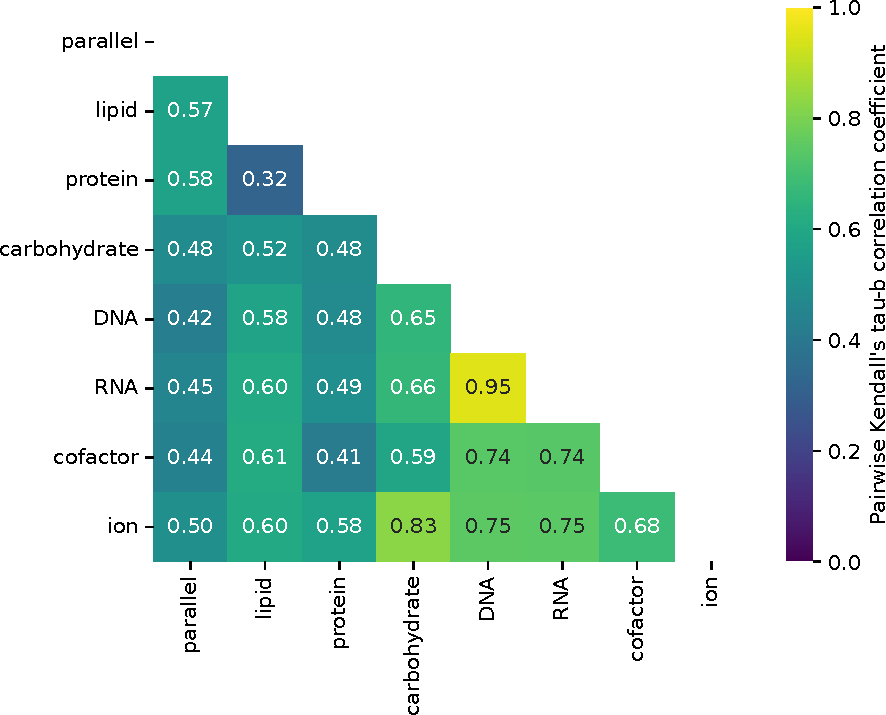
\includegraphics[width=\linewidth]{CompareEnzUse_glc00p00_pyr08p89_ammUnres_2.pdf}
    \caption{
    }
    \label{fig:model-rank-pyr-lowratio-kendall}
  \end{subfigure}

  \caption[
    Changes in enzyme usage reaction flux and Kendall's $\tau$-b rank correlation coefficient for each pair, $\exchrate{pyr}$ = \SI{8.89}{\mmolgdwh}.
  ]{
    For the low $\ratioabl$ condition ($\exchrate{pyr}$ = \SI{8.89}{\mmolgdwh}):
    \textbf{(\ref{fig:model-rank-pyr-lowratio-rank})}
    changes in enzyme usage reaction flux in rounds of ablation.
    Columns show the biomass component prioritised.
    In each column, rows represent enzyme usage reactions, arranged in descending order of flux.
    Colours identify the reactions, with white indicating reactions that carry zero flux in the parallel case.
    \textbf{(\ref{fig:model-rank-pyr-lowratio-kendall})}
    Pairwise Kendall's $\tau$-b rank correlation coefficient \parencite{kendallTREATMENTTIESRANKING1945} for each pair of enzyme usage flux profiles.
  }
  \label{fig:model-rank-pyr-lowratio}
\end{figure}

The use of enzyme usage vectors to explain biomass synthesis scheduling strategies is called into question by the multiplicity of solutions in FBA\@.
Fig.\ \ref{fig:model-noisy} shows that the relationship between exchange rates and measures of similarity between enzyme usage fluxes when carbohydrate was prioritised and when protein was prioritised was not continuous.

\begin{figure}[htb!]
  \centering
  \begin{subfigure}[t]{0.45\textwidth}
  \centering
    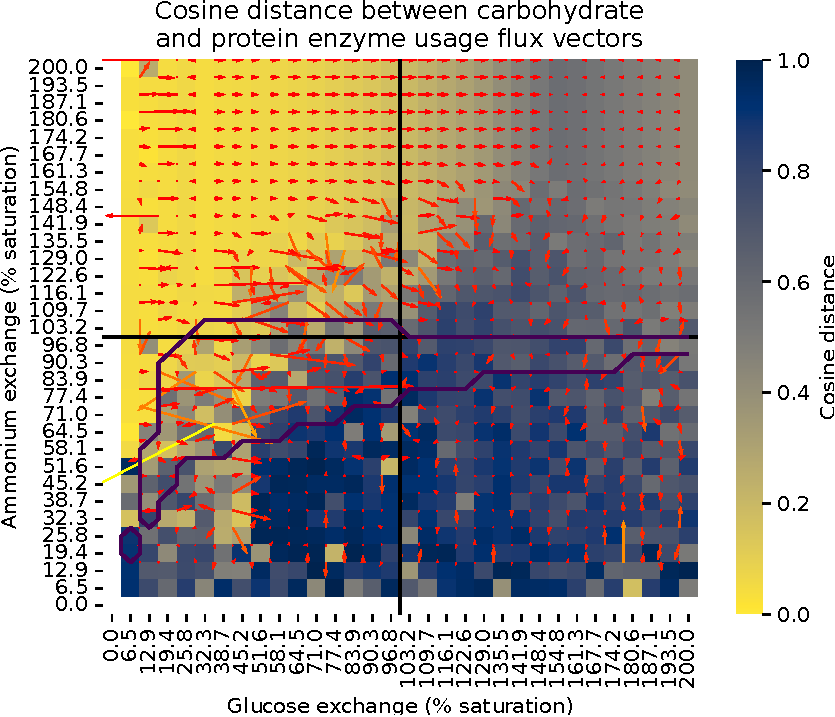
\includegraphics[width=\linewidth]{ec_grid_glc_amm_cosine}
    \caption{
    }
    \label{fig:model-noisy-glc-cosine}
  \end{subfigure}%
  \begin{subfigure}[t]{0.45\textwidth}
  \centering
    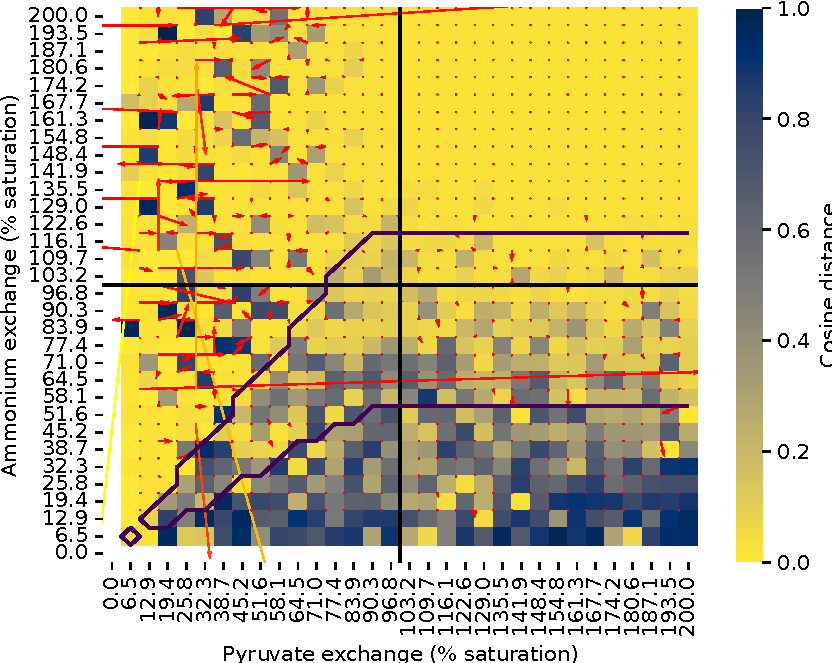
\includegraphics[width=\linewidth]{ec_grid_pyr_amm_cosine}
    \caption{
    }
    \label{fig:model-noisy-pyr-cosine}
  \end{subfigure}

  \begin{subfigure}[t]{0.45\textwidth}
  \centering
    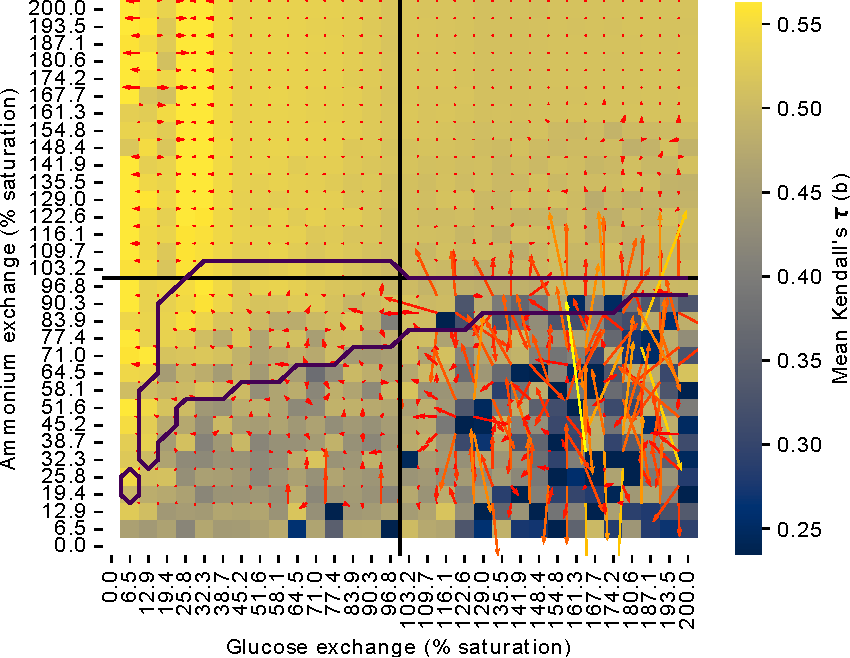
\includegraphics[width=\linewidth]{ec_grid_glc_amm_kendall}
    \caption{
    }
    \label{fig:model-noisy-glc-kendall}
  \end{subfigure}%
  \begin{subfigure}[t]{0.45\textwidth}
  \centering
    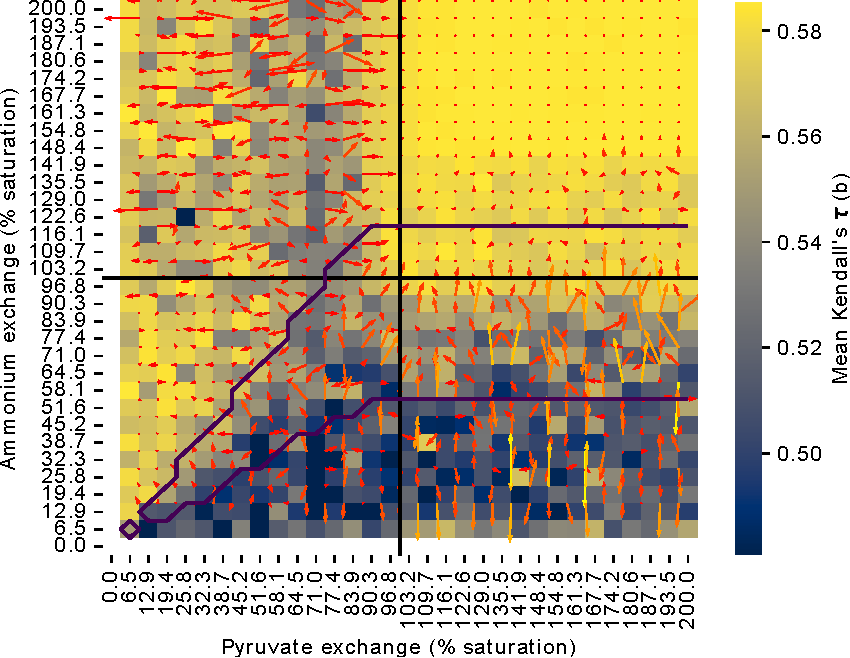
\includegraphics[width=\linewidth]{ec_grid_pyr_amm_kendall}
    \caption{
    }
    \label{fig:model-noisy-pyr-kendall}
  \end{subfigure}

  \caption[
    Measures of similarity between enzyme usage fluxes in different nutrient conditions
  ]{
    Measures of similarity between enzyme usage fluxes in different nutrient conditions.
    Cosine distances between the vector of enzyme usage fluxes when protein is prioritised and the equivalent vector when carbohydrate is prioritised are shown \textbf{(\ref{fig:model-noisy-glc-cosine})} for glucose-ammonium conditions and \textbf{(\ref{fig:model-noisy-pyr-cosine})} pyruvate-ammonium conditions; smaller distances indicate a greater similarity between the two conditions.
    Means of the set of Kendall's $\tau$-b rank correlation coefficients between the parallel case and each biomass-prioritised case are shown \textbf{(\ref{fig:model-noisy-glc-kendall})} for glucose-ammonium conditions and \textbf{(\ref{fig:model-noisy-pyr-kendall})} pyruvate-ammonium conditions; larger mean values indicate a greater similarity between parallel biosynthesis and individual biomass component synthesis.
    }
  \label{fig:model-noisy}
\end{figure}

This observation is likely explained by the multiplicity of solutions in FBA\@.
Namely, while FBA finds the optimal value of the objective function, there is no guarantee that the flux vector $\mathbf{v}$ (Eq.\ \ref{eq:model-fba-objective}) is equivalent across linear programming solvers.
% I still don't like this sentence.
In sum, although choosing representative nutrient conditions led to an attractive picture that may confirm the hypothesis that the cell favours parallel biosynthesis in nutrient limiting conditions if biomass components share metabolic pathways, the computational limitations of FBA may cast doubts on conclusions.


\section{Discussion}
\label{subsec:model-discussion}

This chapter uses a genome-scale model of budding yeast and flux balance analysis to test whether sequential synthesis of biomass components reflects an adaptation to limited cellular resources.
% The cell synthesises its biomass components in sequence, re-allocating its proteome to enzymes that have roles related to the synthesis of each biomass component, as an adaptation to a limited proteome pool.
% However, changes in nutrient conditions may make parallel biosynthesis advantageous if the proteome allocation between biomass components become more similar.

My results suggest that ablation of components of the biomass reaction was a viable method to simulate sequential synthesis of biomass components, as evidenced by how ablation predicted biologically relevant changes in proteome allocation to enzymes.
In addition, ablation led to a way to estimate the time of synthesis of biomass components.
These times suggest that sequential scheduling of biosynthesis saves time during growth and remains advantageous across deletion strains.

My results further show that within realistic growth rates, a smaller proteome pool led to a greater advantage of sequential biosynthesis over parallel biosynthesis.
However, parallel scheduling of biosynthesis becomes advantageous in some nutrient conditions, such as when both carbon and nitrogen sources are limiting.
Further simulations suggest an explanation for this advantage of parallel biosynthesis: as each biomass component is synthesised, the cell allocates its proteome pool to enzymes in similar patterns.

The advantage of sequential scheduling of biosynthesis over parallel scheduling of biosynthesis may explain why yeast cells exhibit metabolic cycles, in which there is a sequence of synthesising biomass components \parencite{mellorMolecularBasisMetabolic2016}.
Conversely, the advantage of parallel scheduling of biosynthesis over sequential scheduling of biosynthesis in nutrient-limiting conditions may explain the absence of metabolic cycles in extreme, non-permissive conditions.
The metabolic cycle may thus be an adaptation to a limited proteome pool and having to carry out the metabolically expensive process of protein synthesis during cell growth \parencite{oneillEukaryoticCellBiology2020}.
Clustering of the synthesis of lipids and proteins in one group may explain cycling of storage lipids \parencite{campbellBuildingBlocksAre2020}, while clustering of carbohydrate, DNA, and RNA synthesis in another group to group together processes that require oxidative phosphorylation may explain respiratory cycles in the YMC \parencite{tuLogicYeastMetabolic2005}.

However, the limitations of using FBA to investigate resource allocation strategies in this chapter include multiplicity of solutions and a lack of ability to preform concentration-dependent, time-dependent, and compartment-dependent simulations.
The multiplicity of solutions in FBA makes it challenging to draw conclusions about how quantities derived from flux values apart from growth.
These values in the GECKO model include enzyme usage reaction fluxes, which would inform proteome allocation strategies.
In addition, FBA gives a steady-state picture of metabolism.
To describe changes in fluxes over time, derivatives such as dynamic FBA \parencite{mahadevanDynamicFluxBalance2002} could be used.
To further increase the precision of the model and thus its ability to make predictions, compartmentalisation can be considered \parencite{elsemmanWholecellModelingYeast2022}, or resource balance analysis \parencite{goelzerCellDesignBacteria2011} can be used.
